%%
%% Copyright 2007, 2008, 2009 Elsevier Ltd
%%
%% This file is part of the 'Elsarticle Bundle'.
%% ---------------------------------------------
%%
%% It may be distributed under the conditions of the LaTeX Project Public
%% License, either version 1.2 of this license or (at your option) any
%% later version.  The latest version of this license is in
%%    http://www.latex-project.org/lppl.txt
%% and version 1.2 or later is part of all distributions of LaTeX
%% version 1999/12/01 or later.
%%
%% The list of all files belonging to the 'Elsarticle Bundle' is
%% given in the file `manifest.txt'.
%%

%% Template article for Elsevier's document class `elsarticle'
%% with numbered style bibliographic references
%% SP 2008/03/01
%%
%%
%%
%% $Id: elsarticle-template-num.tex 4 2009-10-24 08:22:58Z rishi $
%%
%%
\documentclass[final,3p,times,twocolumn]{elsarticle}

%% Use the option review to obtain double line spacing
%% \documentclass[preprint,review,12pt]{elsarticle}

%% Use the options 1p,twocolumn; 3p; 3p,twocolumn; 5p; or 5p,twocolumn
%% for a journal layout:
%% \documentclass[final,1p,times]{elsarticle}
%% \documentclass[final,1p,times,twocolumn]{elsarticle}
%% \documentclass[final,3p,times]{elsarticle}
%% \documentclass[final,3p,times,twocolumn]{elsarticle}
%% \documentclass[final,5p,times]{elsarticle}
%% \documentclass[final,5p,times,twocolumn]{elsarticle}

\usepackage{amssymb}
\usepackage{amsfonts}
\usepackage{graphicx}%[dvips]
\usepackage{amsmath}
\usepackage{latexsym}
\usepackage{pstricks}
\usepackage{mathrsfs}

\newcommand{\bfxi}{\mbox{\boldmath $\xi$}}
\newcommand{\bfnu}{\mbox{\boldmath $\nu$}}
\newcommand{\bflam}{\mbox{\boldmath $\Lambda$}}
\newcommand{\bfphi}{\mbox{\boldmath $\varphi$}}
\newcommand{\bfpsi}{\mbox{\boldmath $\psi$}}
\newcommand{\bfc}{\mbox{\boldmath $c$}}
\newcommand{\bfd}{\mbox{\boldmath $d$}}
\newcommand{\bfm}{\mbox{\boldmath $m$}}
\newcommand{\bfx}{\mbox{\boldmath $x$}}
\newcommand{\bfr}{\mbox{\boldmath $r$}}
\newcommand{\bfR}{\mbox{\boldmath $R$}}
\newcommand{\bfv}{\mbox{\boldmath $v$}}
\newcommand{\bfy}{\mbox{\boldmath $y$}}
\newcommand{\bfz}{\mbox{\boldmath $z$}}
\newcommand{\bfu}{\mbox{\boldmath $u$}}
\newcommand{\bfS}{\mbox{\boldmath $S$}}
\newcommand{\bft}{\mbox{\boldmath $t$}}
\newcommand{\bfn}{\mbox{\boldmath $n$}}
\newcommand{\bfM}{\mbox{\boldmath $M$}}
\newcommand{\bfY}{\mbox{\boldmath $Y$}}
\newcommand{\bfX}{\mbox{\boldmath $X$}}
\newcommand{\bfC}{\mbox{\boldmath $C$}}


%%%%%%%%%%%%%new commands%%%%%%%%%%%%%%%%%%%%%%%%%%%%%%%%%%%%%%
\newenvironment{proof}[1][Proof]{\begin{trivlist}
\item[\hskip \labelsep {\bfseries #1}]}{\end{trivlist}}
\newenvironment{definition}[1][Definition]{\begin{trivlist}
\item[\hskip \labelsep {\bfseries #1}]}{\end{trivlist}}
\newenvironment{example}[1][Example]{\begin{trivlist}
\item[\hskip \labelsep {\bfseries #1}]}{\end{trivlist}}

\newcommand{\icom}{{\mbox{\rm $\scriptscriptstyle ^\mid$\hspace{-0.40em}C}}}
\newcommand{\om}{\Omega}
\newcommand{\pom}{\partial\Omega}
\newcommand{\epal}{{\mathcal E}(\overline{\om})}
\newcommand{\ak}{A_k}
\newcommand{\bk}{B_k}
\newcommand{\buuv}{b(\bfu,\bfu,\bfv)}
\newcommand{\buwt}{b(\bfu,\bfw,.)}
\newcommand{\buwv}{b(\bfu,\bfw,\bfv)}
\newcommand{\bwuv}{b(\bfw,\bfu,\bfv)}
\newcommand{\cco}{c = c(\om)}
\newcommand{\ccot}{c = c(\om,T)}
\newcommand{\cd}{c_2}
\newcommand{\cdco}{c_2 = c_2(\om)}
\newcommand{\cj}{c_1}
\newcommand{\cjco}{c_1 = c_1(\om)}
\newcommand{\cjcot}{c_1 = c_1(\om,T)}
\newcommand{\ct}{c_3}
\newcommand{\ctco}{c_3 = c_3(\om)}
\newcommand{\cy}{c_4}
\newcommand{\cyco}{c_4 = c_4(\om)}
\newcommand{\ddt}{{{d}\over{dt}}}
\newcommand{\dom}{\mbox{ }d(\om)}
\newcommand{\ds}{\mbox{ }ds}
\newcommand{\dt}{\mbox{ }dt}
\newcommand{\dpg}{\mbox{ }d(\partial\om)}
\newcommand{\dc}{\|}
\newcommand{\dz}{\bigl(\!\bigl(}
\newcommand{\bdz}{(\!(}
\newcommand{\dzr}{)\!)}
\newcommand{\eij}{e_{ij}}
\newcommand{\eiju}{e_{ij}(\bfu)}
\newcommand{\eijv}{e_{ij}(\bfv)}
\newcommand{\eijw}{e_{ij}(\bfw)}
\newcommand{\eu}{{\mathcal A}_u}
\newcommand{\fk}{f_k}
\newcommand{\fn}{f_0}
\newcommand{\gj}{\Gamma_1}
\newcommand{\gd}{\Gamma_2}
\newcommand{\gh}{{\mathcal G}_H}
\newcommand{\gv}{{\mathcal G}}
\newcommand{\gt}{\Gamma_3}
\newcommand{\gc}{\Gamma_4}
\newcommand{\ha}{H}
\newcommand{\haa}{H}
\newcommand{\intnt}{\int_0^T}
\newcommand{\intnst}{\int_0^{T^*}}
\newcommand{\iom}{\int_\om}
\newcommand{\isom}{\int_{\partial\om}}
\newcommand{\kc}{K_C}
\newcommand{\pcx}{P_c}
\newcommand{\ldd}{L^2(0,T;\,D)}
\newcommand{\ldsd}{L^2(0,\ts;\,D)}
\newcommand{\ldh}{L^2(0,T;\,H)}
\newcommand{\ldsh}{L^2(0,\ts;\,H)}
\newcommand{\ldon}{L^2(\om)^m}
\newcommand{\ldv}{L^2(0,T;\,\vajd)}
\newcommand{\ldsv}{L^2(0,\ts;\,\vajd)}
\newcommand{\ldvso}{L^2(0,T;\,\vso)}
\newcommand{\lnvso}{L^{\infty}(0,T;\,\vso)}
\newcommand{\lnv}{L^{\infty}(0,T;\,\vajd)}
\newcommand{\lnsv}{L^{\infty}(0,\ts;\,\vajd)}
\newcommand{\lnvh}{L^{\infty}(0,T;\,\vajdh)}
\newcommand{\ldvh}{L^2(0,T;\,\vajdh)}
\newcommand{\lnh}{L^\infty(0,T;\,H)}
\newcommand{\lno}{L^\infty(\om)^3}
\newcommand{\lco}{L^4(\om)^m}
\newcommand{\ldor}{L^2(\om)/\iree}
\newcommand{\mc}{{\mathcal M}_C}
\newcommand{\mn}{M_0}
\newcommand{\mr}{{\mathcal M}_R}
\newcommand{\nd}{\|_D}
\newcommand{\njd}{\|_{V^{1,2}}}
\newcommand{\nnd}{\|_{H}}
\newcommand{\njp}{\|_{V^{1,p}}}
\newcommand{\njq}{\|_{V^{1,q}}}
\newcommand{\njqh}{\|_{({V^{1,q}})^*}}
\newcommand{\nldd}{\|_{L^2(0,T;\,D)}}
\newcommand{\nldv}{\|_{\ldv}}
\newcommand{\nldvh}{\|_{L^2(0,T;\,\vajd^*)}}
\newcommand{\nlnv}{\|_{\lnv}}
\newcommand{\nlnvso}{\|_{L^\infty(0,T;\,\vajd^{{7/8},2})}}
\newcommand{\nldvso}{\|_{L^2(0,T;\,\vajd^{{7/8},2})}}
\newcommand{\nlnvh}{\|_{\lnvh}}
\newcommand{\nldh}{\|_{L^2(0,T;\,H)}}
\newcommand{\nlnh}{\|_{L^\infty(0,T;\,\haa)}}
\newcommand{\nha}{\|_{\haa}}
\newcommand{\nlco}{\|_{\lco}}
\newcommand{\nre}{\|_E}
\newcommand{\nt}{(0,T)}
\newcommand{\nv}{\|_V}
\newcommand{\nvjdh}{\|_{\vajdh}}
\newcommand{\nvso}{\|_{\vso}}
\newcommand{\nvrd}{\|_{\vrd}}
\newcommand{\nvnth}{\|_{\vnth}}
\newcommand{\nwjd}{\|_{\wjdo}}
\newcommand{\nwkd}{\|_{\wkd}}
\newcommand{\nx}{\|_X}
\newcommand{\nxj}{\|_{\xj}}
\newcommand{\nxd}{\|_{\xd}}
\newcommand{\nxp}{\|_{\xp}}
\newcommand{\ny}{\|_{X_2}}
\newcommand{\nyp}{\|_{\yp}}
\newcommand{\ob}{{\mathcal B}}
\newcommand{\obp}{{\mathcal B}_{\mathcal P}}
\newcommand{\oc}{{\mathcal C}}
\newcommand{\ocp}{{\mathcal C}_{\mathcal P}}
\newcommand{\ogu}{{\mathcal G}_u}
\newcommand{\ogpu}{{{\mathcal G}_{\mathcal P}}_{\bfu}}
\newcommand{\oh}{{\cal H}}
\newcommand{\ohj}{{\cal H}_1}
\newcommand{\ohd}{{\cal H}_2}
\newcommand{\oht}{{\cal H}_3}
\newcommand{\okc}{\overline{\kc}}
\newcommand{\oku}{{\cal K}_u}
\newcommand{\okpu}{{{\cal K}_{\cal P}}_{\bfu}}
\newcommand{\omnt}{\om\times\nt}
\newcommand{\omu}{\bfgamma_0}
\newcommand{\on}{{\cal N}}
\newcommand{\onp}{{\cal N}_{\cal P}}
\newcommand{\pres}{{\cal P}}
\newcommand{\pu}{P;\bfu}
\newcommand{\phik}{\bfPhi_k}
\newcommand{\psik}{\bfPsi_k}
\newcommand{\sh}{\bigr)\!\bigr)_H}
\newcommand{\bsh}{\Bigr)\!\Bigr)_H}
\newcommand{\bshaa}{\bigr)\!\bigr)_{0,2}}
\newcommand{\swnjdo}{)\!)_{\wnjdo}}
\newcommand{\sd}{)\!)_D}
\newcommand{\svjd}{)\!)_V}
\newcommand{\svajd}{\bigr)\!\bigr)_V}
\newcommand{\bsvjd}{\bigr)\!\bigr)_V}
\newcommand{\bsvajd}{\bigr)\!\bigr)_{1,2}}
\newcommand{\sldv}{)\!)_{\ldv}}
\newcommand{\sumkjinf}{\sum_{k=1}^{\infty}}
\newcommand{\os}{{\cal S}}
\newcommand{\osp}{{\cal S}_{\cal P}}
\newcommand{\tc}{\|}
\newcommand{\ts}{T^*}
\newcommand{\tnt}{t\in(0,T)}
\newcommand{\tnts}{t\in(0,\ts)}
\newcommand{\ud}{\bfu_B}
\newcommand{\uj}{{\bfu}_A}
\newcommand{\uk}{\bfu_k}
\newcommand{\unu}{{\bfu}_0}
\newcommand{\vjd}{V}
\newcommand{\vajd}{V}
\newcommand{\vakp}{V^{k,p}}
\newcommand{\vajdh}{\vajd^*}
\newcommand{\vso}{V_\kappa^{{7/8},2}}
\newcommand{\vrd}{V^{r_0,2}}
\newcommand{\vvajd}{\bfv\in\vajd}
\newcommand{\vnq}{V^{0,q}}
\newcommand{\vnt}{V^{0,3}}
\newcommand{\vnth}{(V^{0,3})^*}
\newcommand{\wjdo}{W^{1,2}(\om)^m}
\newcommand{\wnjdo}{W_0^{1,2}(\om)}
\newcommand{\wnjdoh}{W_0^{1,2}(\om)^*}
\newcommand{\wnjdon}{W_0^{1,2}(\om)^m}
\newcommand{\wnjdonh}{(W_0^{1,2}(\om)^m)^*}
\newcommand{\wjdp}{W^{1,{12/5}}(\om)}
\newcommand{\wk}{\bfw_k}
\newcommand{\wkd}{W^{k,2}(\om)^m}
\newcommand{\wkci}{\bfw_{k,i}}
\newcommand{\wkcj}{\bfw_{k,j}}
\newcommand{\wki}{\bfw_{k_i}}
\newcommand{\wsi}{{\bf w^*_i}}
\newcommand{\wsj}{{\bf w^*_j}}
\newcommand{\nwjdp}{\|_{\wjdp}}
\newcommand{\xp}{X_{\cal P}}
\newcommand{\xv}{X}
\newcommand{\xj}{X_{1,\ts}}
\newcommand{\xd}{X_{2,\ts}}
\newcommand{\yp}{X_2_{\cal P}}
\newcommand{\yv}{X_2}
\newcommand{\zrx}{\bfzero_X}
\newcommand{\zry}{\bfzero_{X_2}}
\newcommand{\zrxp}{\bfzero_{\xp}}
\newcommand{\zryp}{\bfzero_{\yp}}
\newcommand{\bfb}{\mbox{\boldmath{$b$}}}
% \newcommand{\bfx}{\mbox{\boldmath{$x$}}}
% \newcommand{\bfn}{\mbox{\boldmath{$n$}}}
\newcommand{\bfe}{\mbox{\boldmath{$e$}}}
\newcommand{\bff}{\mbox{\boldmath{$f$}}}
\newcommand{\bfF}{\mbox{\boldmath{$F$}}}
\newcommand{\bfg}{\mbox{\boldmath{$g$}}}
\newcommand{\bfq}{\mbox{\boldmath{$q$}}}
\newcommand{\bfh}{\mbox{\boldmath{$h$}}}
% \newcommand{\bfu}{\mbox{\boldmath{$u$}}}
\newcommand{\bfw}{\mbox{\boldmath{$w$}}}
% \newcommand{\bfv}{\mbox{\boldmath{$v$}}}
% \newcommand{\bfz}{\mbox{\boldmath{$z$}}}
\newcommand{\bfL}{\mbox{\boldmath{$L$}}}
\newcommand{\bfa}{\mbox{\boldmath{$a$}}}
% \newcommand{\bfU}{\mbox{\boldmath{$U$}}}
% \newcommand{\bfM}{\mbox{\boldmath{$M$}}}
\newcommand{\bfN}{\mbox{\boldmath{$N$}}}
\newcommand{\bfE}{\mbox{\boldmath{$E$}}}
% \newcommand{\bfC}{\mbox{\boldmath{$C$}}}
% \newcommand{\bfS}{\mbox{\boldmath{$S$}}}
\newcommand{\bfJ}{\mbox{\boldmath{$J$}}}
% \newcommand{\bfy}{\mbox{\boldmath{$y$}}}
\newcommand{\bfp}{\mbox{\boldmath{$p$}}}
\newcommand{\bfK}{\mbox{\boldmath{$K$}}}
\newcommand{\bfI}{\mbox{\boldmath{$I$}}}
\newcommand{\bfP}{\mbox{\boldmath{$P$}}}
\newcommand{\bfB}{\mbox{\boldmath{$B$}}}
\newcommand{\bfH}{\mbox{\boldmath{$H$}}}
\newcommand{\bfV}{\mbox{\boldmath{$V$}}}
\newcommand{\bfW}{\mbox{\boldmath{$W$}}}
% \newcommand{\bfD}{\mbox{\boldmath{$D$}}}
% \newcommand{\bfR}{\mbox{\boldmath{$R$}}}
\newcommand{\bfmathcalF}{\mbox{\boldmath{$\mathcal{F}$}}}
\newcommand{\bfmathcalA}{\mbox{\boldmath{$\mathcal{A}$}}}
% \newcommand{\bfX}{\mbox{\boldmath{$X$}}}
\newcommand{\bfmu}{\mbox{\boldmath{$\mu$}}}
\newcommand{\bflambda}{\mbox{\boldmath{$\lambda$}}}
\newcommand{\bfomega}{\mbox{\boldmath{$\omega$}}}
% \newcommand{\bfphi}{\mbox{\boldmath{$\phi$}}}
\newcommand{\bfeta}{\mbox{\boldmath{$\eta$}}}
\newcommand{\bftau}{\mbox{\boldmath{$\tau$}}}
\newcommand{\bfPhi}{\mbox{\boldmath{$\Phi$}}}
% \newcommand{\bfpsi}{\mbox{\boldmath{$\psi$}}}
\newcommand{\bftheta}{\mbox{\boldmath{$\theta$}}}
\newcommand{\bfPsi}{\mbox{\boldmath{$\Psi$}}}
\newcommand{\bfT}{\mbox{\boldmath{${\cal T}$}}}
\newcommand{\bfTheta}{\mbox{\boldmath{$\Theta$}}}
\newcommand{\bfsigma}{\mbox{\boldmath{$\sigma$}}}
\newcommand{\bfvarsigma}{\mbox{\boldmath{$\varsigma$}}}
\newcommand{\bfupsilon}{\mbox{\boldmath{$\upsilon$}}}
\newcommand{\bfgamma}{\mbox{\boldmath{$\gamma$}}}
\newcommand{\bfvarphi}{\mbox{\boldmath{$\varphi$}}}
\newcommand{\bfzeta}{\mbox{\boldmath{$\zeta$}}}
\newcommand{\bfchi}{\mbox{\boldmath{$\chi$}}}
% \newcommand{\bft}{\mbox{\boldmath{$t$}}}
\newcommand{\bfmathcalp}{\mbox{\boldmath{$\mathcal{p}$}}}
\newcommand{\bfLambda}{\mbox{\boldmath{$\Lambda$}}}
\newcommand{\bfzero}{{\bf 0}}
\newcounter{constants}
\setcounter{constants}{0}
\newcommand{\cn}[2]{ \addtocounter{constants}{1} \newcounter{c#1#2}
\setcounter{c#1#2}{\value{constants}} c_{\arabic{c#1#2}} }
\newcommand{\cc}[2]{c_{\arabic{c#1#2}}}
\newcommand{\MBtext}[1]{\marginpar{\red \scriptsize $\leftarrow$ #1}}

%%%%%%%%end new commands%%%%%%%%%%%%%%%%%%%%%%%%%%%%%%%%%%%%


\usepackage{fancyvrb}
\DefineVerbatimEnvironment{code}{Verbatim}{fontsize=\footnotesize}
\DefineVerbatimEnvironment{example}{Verbatim}{fontsize=\footnotesize}
%\usepackage{listings}
%\lstset{language=C++}
%\lstset{frame=shadowbox, rulesepcolor=\color{blue}}

%% if you use PostScript figures in your article
%% use the graphics package for simple commands
%% \usepackage{graphics}
%% or use the graphicx package for more complicated commands
%% \usepackage{graphicx}
%% or use the epsfig package if you prefer to use the old commands
%% \usepackage{epsfig}

%% The amssymb package provides various useful mathematical symbols
\usepackage{amssymb}
\usepackage{graphicx}
%% The amsthm package provides extended theorem environments
%% \usepackage{amsthm}

%% The lineno packages adds line numbers. Start line numbering with
%% \begin{linenumbers}, end it with \end{linenumbers}. Or switch it on
%% for the whole article with \linenumbers after \end{frontmatter}.
%% \usepackage{lineno}

%% natbib.sty is loaded by default. However, natbib options can be
%% provided with \biboptions{...} command. Following options are
%% valid:

%%   round  -  round parentheses are used (default)
%%   square -  square brackets are used   [option]
%%   curly  -  curly braces are used      {option}
%%   angle  -  angle brackets are used    <option>
%%   semicolon  -  multiple citations separated by semi-colon
%%   colon  - same as semicolon, an earlier confusion
%%   comma  -  separated by comma
%%   numbers-  selects numerical citations
%%   super  -  numerical citations as superscripts
%%   sort   -  sorts multiple citations according to order in ref. list
%%   sort&compress   -  like sort, but also compresses numerical citations
%%   compress - compresses without sorting
%%
%% \biboptions{comma,round}

% \biboptions{}


\journal{Advanced Water Resources}

\begin{document}

\begin{frontmatter}

%% Title, authors and addresses

%% use the tnoteref command within \title for footnotes;
%% use the tnotetext command for the associated footnote;
%% use the fnref command within \author or \address for footnotes;
%% use the fntext command for the associated footnote;
%% use the corref command within \author for corresponding author footnotes;
%% use the cortext command for the associated footnote;
%% use the ead command for the email address,
%% and the form \ead[url] for the home page:
%%
%% \title{\tnoteref{label1}}
%% \tnotetext[label1]{}
%% \author{Name\corref{cor1}\fnref{label2}}
%% \ead{email address}
%% \ead[url]{home page}
%% \fntext[label2]{}
%% \cortext[cor1]{}
%% \address{Address\fnref{label3}}
%% \fntext[label3]{}

\title{Solving the Nonstationary Richards Equation\\
       With Adaptive $hp$-FEM}

%% use optional labels to link authors explicitly to addresses:
%% \author[label1,label2]{<author name>}
%% \address[label1]{<address>}
%% \address[label2]{<address>}

\author{Pavel Solin$^{1,2}$, Michal Kuraz$^3$}

\address{${}^1$Department of Mathematics and Statistics, University of Nevada, Reno, USA}
\address{${}^2$Institute of Themomechanics, Prague, Czech Republic}
\address{${}^3$Department of Water Resources and Environmental Modeling, Czech University of Life Sciences Prague, Czech Republic}
%\address{${}^4$Institute of Physics, Academy of Sciences of the Czech Republic, Czech Republic}

\begin{abstract}
%% Text of abstract
This paper examines the potential of the adaptive $hp$-FEM method for the 
numerical solution of time-dependent variably saturated 
Darcian flow problems described by the Richards equation. The method is 
illustrated on three model problems: a benchmark with known exact solution, 
groundwater seepage into a dry lysimeter box with time-dependent boundary 
conditions, and capillary barrier behavior under an intense infiltration. 
In the second part of the paper we present the weak formulation of the Richards equation 
for the Newton's and Picard's methods, give a brief overview of adaptive 
$hp$-FEM with emphasis on aspects that are usually not discussed in the 
literature, and we briefly introduce the open source adaptive $hp$-FEM library 
HERMES that was used to generate numerical results for this paper. All 
computations that we present are easily reproducible.
\end{abstract}

\begin{keyword}
%% keywords here, in the form: keyword \sep keyword
Richards equation \sep Adaptive $hp$-FEM \sep Dynamically-changing meshes \sep Reproducible research

%% MSC codes here, in the form: \MSC code \sep code
%% or \MSC[2008] code \sep code (2000 is the default)

\end{keyword}

\end{frontmatter}

%%
%% Start line numbering here if you want
%%
% \linenumbers

%% main text

\section{Introduction}
\label{sec:intro}

The problem of predicting flow in an unsaturated/saturated zone is 
important in many fields ranging from agriculture and hydrology to technical 
applications such as contaminant transport, disposal of dangerous waste in deep 
rock formations, and others.

The Richards equation is obtained by combining the Darcy-Buckingham's law
with the law of conservation of mass. Its numerical solution 
is the subject of an intense research since the early 1970s, beginning with Neuman's 
finite element solution of unsteady dam seepage~\cite{neuman1}. 
%Celia's mass 
%conservative modified Picard iteration~\cite{celia} method in the early 1990s, 
% the recent Kees's work with focus on stabilized finite element 
%approximations~\cite{kees,kees2,kees3}.
Numerical methods for the Richards equation
can be tested on several simplified examples with known exact solutions 
such as \cite{tracy1,tracy2}. 

It is well known that a straightforward application of the Galerkin approximation
to the Richards equation may yield poor results, especially when coarse meshes are 
used in areas with steep gradients such as wetting fronts.
Often this is due to large values of the convective term 
$\frac{\partial K(h)}{\partial z}$, where $K(h)$ is unsaturated hydraulic 
conductivity, that cause stability problems.
It follows from the relation  $\frac{\partial K(h)}{\partial z}=K'(h)\frac{\partial h}{\partial z}$
that the problems are in fact caused by large slopes of $K(h)$. 

One of the goals of this paper is to show that to a certain extent, these problems 
can be avoided by resolving areas with steep solution gradients with adaptive 
finite element methods, so that 
the underlying reason for the nonphysical oscillations ceases to exist. In particular,
we focus on the application of adaptive $hp$-FEM, a modern version of the finite element 
method that is capable of extremely fast, exponential convergence \cite{babuska1}
(subject to certain assumptions on the solution of the problem which do not exclude
singular solutions and solutions with steep gradients).


%tady jsem konkretni cisla section zmenil na odkaz na sekci, vysazene to vypada stejne
The outline of the paper is as follows: To make the paper self-contained and to 
establish notation, in Section~\ref{sec:richards} we introduce the Richards equation and 
relevant constitutive relations. In Section~\ref{sec:hpfem} we
demonstrate the potential of adaptive $hp$-FEM using an elliptic benchmark problem with known 
exact solution. In Section~\ref{sec:compar}, an analogous comparison with low-order finite element 
methods is done for the time-dependent Richards equation, in the context of a 
benchmark problem with known exact solution. Section~\ref{sec:example} is dedicated to solving 
with adaptive $hp$-FEM a nonstationary groundwater seepage into a dry lysimeter box,
with time-dependent boundary conditions. Section~\ref{sec:example-barrier} deals with 
a nonstationary problem of capillary barrier behavior under an intense infiltration into 
an initially unsaturated medium. Conclusions and outlook are drawn in Section \ref{sec:8}.

In Appendix A we present weak forms for the Richards equation and their solution 
via the Picard's and Newton's methods, describe in more detail some particular 
aspects on adaptive 
$hp$-FEM that are relevant for computations performed in this paper. In Appendix B we
briefly introduce the open source adaptive $hp$-FEM library HERMES \cite{hermes} 
that was used to generate numerical results for this paper. 


\section{Richards Equation}
\label{sec:richards}


The mathematical model of  unsaturated flow was originally published in \cite{richards}. 
This formula, usually identified as the  mixed form of the Richards equation,  states that 

\begin{equation}
\label{mixed}
\frac{\partial \theta}{\partial t} - \nabla \cdot \left( K(\theta) \nabla h \right) - \frac{\partial K(\theta)}{\partial z} = 0.
\end{equation}
Here $\theta$ is the water content of a porous material [-], $h$ is the pressure head [$L$],  $K(\theta)$ is the unsaturated hydraulic conductivity function [$L.T^{-1}$],  $z$ denotes the 
vertical dimension [$L$], assumed positive upwards, and the porous medium is assumed to be isotropic. Appropriate  constitutive
relationships among $\theta$ and $h$, $K$ and~$h$, are also assumed.

This PDE can be generalized as a quasilinear elliptic-parabolic differential equation and as 
a degenerate convection-diffusion problem. A proof of the existence of a   solution  is given in~\cite{alt-luckhaus}. 

This model is applicable to unsteady unsaturated flow, thus for $h \in (-\infty , 0 \rangle$. 
An extension into saturated zone can be obtained by modifying the time derivative term 
as considered in Neumann's and Huyakorn's works (see, e.g.,~\cite{neuman1,neuman2,neuman3,huyakorn1,huyakorn2}). The modification has the form 

\begin{equation}
\label{neuman-mod}
\frac{\partial \theta}{\partial t} + \frac{\theta}{\theta_S} S \frac{\partial h}{\partial t}
- \nabla \cdot \left( K(\theta) \nabla h \right) - \frac{\partial K(\theta)}{\partial z} = 0,
\end{equation}
where $\theta_S$ is the saturated water content [-] and $S$ the specific storativity 
[$L^{-1}$]. Such an approach is suitable, e.g., for modeling an unsteady dam seepage.
%vetu "Equation (\ref{neuman-mod})  can also be assumed in the standard $h$-based form,"
%nahrazuji nasledujicim (protoze rovnice na kterou se odkazuje NENI h-based)
%ta posledni je h-based
The time derivative term of the water content function can be substituted by 
the so called retention water capacity ($C(h) = \frac{\textrm{d}\theta}{\textrm{d} h}$ [$L^{-1}$])
in order to obtain the standard $h$-based form

\begin{equation}\label{rich-final}
\left(C(h)
+ \frac{\theta}{\theta_S} S \right) \frac{\partial h}{\partial t}
- \nabla \cdot \left( K(h) \nabla h \right) - \frac{\partial K(h)}{\partial z} = 0.\ \ \ \ 
\end{equation}

\subsection{Constitutive Relations}

A relation between the water content and the pressure head is called 
a {\em retention curve}. Its most commonly used analytical formula is 
the van Genuchten's equation~\cite{vangenuchten}:

\begin{equation}
\label{vangenuchten-eq}
\theta (h) = \left\{ 
\begin{array}{l l}
 \frac{\theta_s -\theta_r}{(1+(-\alpha |h|)^n)^m} + \theta_r,  & \quad \mbox{$\forall$ $h \in (-\infty, 0 )$}\\
  \theta_S, & \quad \mbox{$\forall$ $h \in \langle 0, + \infty )$}.\\
\end{array} \right.
\end{equation}
Here $\alpha$ [$L^{-1}$] is an empirical parameter  whose inverse is often 
referred to as the air entry value or bubbling pressure, and $n$ and $m$ [-]  
are a pore-size distribution parameters affecting the slope of the retention 
function.

The relation between the hydraulic conductivity and the negative pressure head, an 
unsaturated conductivity function, might be defined by the Mualem's model~\cite{mualem}:

  \begin{equation}
  \label{mualem-int}
  K(h) = \left\{
    \begin{array}{l l}
     K_s \sqrt{ \left( \frac{\theta}{\theta_s} \right)} \left( \frac{\int\limits_{\theta_r}^{\theta} \frac{1}{h(\theta)}d \theta }{\int\limits_{\theta_r}^{\theta_S} \frac{1}{h(\theta)} d \theta} \right)^2  \\
    \mbox{$\forall \theta \in (\theta_r, \theta_S )$ $\Rightarrow$ $h \in$ $(-\infty,0)$}; \\
    K_s \ \mbox{$\forall \theta= \theta_S $  $\Rightarrow$  $h \in$ $\langle 0, +\infty)$}.\\
    \end{array} \right.
    \end{equation}
Here $\theta_r$ is the so called {\em residual water content} [-] -- a bottom 
limit of water content for Darcian flow to occur, $K_s$ is the saturated 
hydraulic conductivity (the maximum value).


%odkomentoval jsem, protoze se na tuto analytickou rovnici budu dal v textu odkazovat
When van Genuchten's formula (\ref{vangenuchten-eq}) is substituted into this integral 
law, the following analytical formula is obtained

  \begin{equation}
  \label{mualem-anal}
  K(h) = \left\{
    \begin{array}{l l}
    K_s \frac{\left( 1- (-\alpha h)^{nm} \left( 1+ (-\alpha h)^n \right)^{-m} \right)^2}{\left(1+(-\alpha h)^n \right)^{\frac{m}{2}}} \\
    \mbox{$\forall$ $h \in$ $(-\infty,0)$};\\
    K_s  \ \mbox{$\forall$ $h \in$ $\langle 0, +\infty)$}\\
    \end{array} \right.
    \end{equation}
%%%%%%%%%%%%%%%%%%%%%%%%%%%%%%%%%%%%%%%%%%%%%%%%%%%%%%%%%%%%%

Due to the great complexity of the van Genuchten's relations (\ref{vangenuchten-eq}) 
and (\ref{mualem-int}), an older exponential Gardner's model~\cite{gardner} 
is sometimes used in works treating analytical aspects such as, e.g.,~\cite{tracy1,tracy2}. 
The Gardner's model has the form

\begin{equation}
\label{gardner-theta}
\theta (h) = \left\{ 
\begin{array}{l l}
 \theta_r + (\theta_s -\theta_r)\textrm{e}^{\alpha h}. & \mbox{$\forall$  $h \in$ $(-\infty,0)$},\\
  \theta_S, & \mbox{$\forall$ $h \in \langle 0, + \infty )$},
\end{array} \right.
\end{equation}
and 

  \begin{equation}
  \label{gardner-K}
  K(h) = \left\{
    \begin{array}{l l}
    K_s \textrm{e}^{\alpha h},  &  \mbox{$\forall$  $h \in$ $(-\infty,0)$},\\
    K_s, & \mbox{$\forall$   $h \in$ $\langle 0, +\infty)$}.
    \end{array} \right.
    \end{equation}




\section{Adaptive $hp$-FEM}
\label{sec:hpfem}

The finite element method (FEM) is the most widely used numerical technique
to solve partial differential equations (PDE). 
By adaptive $hp$-FEM we mean a modern version of FEM that combines
adaptively finite elements of different spatial diameters $(h)$ and polynomial
degrees $(p)$ in order to maximize the convergence rate.
For theory and technical details of higher-order FEM
and automatic $hp$-adaptivity we refer, e.g., to \cite{sosedo} 
and many references therein. In the following let us present
a simple example that illustrates the large computational potential of 
the method. 

We solve a standard benchmark problem for adaptive finite element 
methods (see, e.g., \cite{sode}) that 
assumes the Laplace equation $-\Delta u = 0$ in an L-shape domain
$\Omega = (-1, 1)^2 \setminus [-1, 0]^2$. This problem comes with an exact 
solution which is harmonic in $\Omega$ but exhibits a singularity at the 
re-entrant corner:

$$
u(x,y) = r^{2/3} \sin(2 \theta / 3 + \pi / 3).
$$
Here, $(r, \theta)$ are standard polar coordinates. The problem has 
Dirichlet boundary conditions that are given by the exact solution. 
The function $u(x, y)$ is shown in Fig. \ref{fig:lshape-exact}. 


\begin{figure}[!ht]
\begin{center}
\includegraphics[height=4cm]{lshape-exact.png}
\end{center}
\vspace{-4mm}
\caption{Exact solution $u$.}
\label{fig:lshape-exact}
\end{figure}

Note that having an exact solution allows us to calculate the approximation 
error very accurately, and thus compare fairly the performance of different methods. 
The problem will be solved using adaptive $hp$-FEM, adaptive $h$-FEM with 
quadratic elements $(p = 2)$, and adaptive $h$-FEM with linear elements $(p = 1)$
using the open-source finite element library HERMES\footnote{http://hpfem.org/hermes}. 
The library will be described in more detail in Appendix B. 

The three computations start from the same coarse mesh and they are stopped when the 
approximation error drops below $10^{-4}\%$ or when the memory for the matrix solver 
runs out. Therefore each method stops with a different number of degrees of freedom (DOF) and
accuracy, as shown in Table \ref{table:1}.

\begin{table}[!ht]
\begin{center}
\begin{tabular}{|c|c|c|c|}
\hline
Method & DOF & error [\%]\\
\hline
\hline
$h$-FEM $(p=1)$ & 85934 &  $0.094539360$\\
\hline
$h$-FEM $(p=2)$ &115429  & $0.000833918$\\
\hline
$hp$-FEM & 5215 &          $0.000067175$\\
\hline
\end{tabular}
\end{center}
\vspace{-4mm}
\caption{Performance comparison of the three methods.}
\label{table:1}
\end{table}

Fig. \ref{fig:smooth-iso-5} presents a more complete 
convergence comparison of the three methods, and it also 
shows that each method attained its theoreticaly predicted 
asymptotic convergence rate: $h$-FEM with linear 
and quadratic elements have on a log-log convergence 
graph slopes $-1/2$ and $-1$, respectively, and the 
convergence of $hp$-FEM is exponential. A simple extrapolation 
of the linear log-log curves reveals that approx. $10^6$ 
and $10^{12}$ DOF would be needed by the $h$-FEM with quadratic
and linear elements, respectively, to reach the same level of  
accuracy that the $hp$-FEM attained with approx. 5000 DOF.

\begin{figure}[!ht]
\begin{center}
\includegraphics[height=6.2cm]{lshape-conv-dof.png}
\end{center}
\vspace{-8mm}
\caption{Convergence in terms of DOF.}
\label{fig:smooth-iso-5}
%\vspace{-1mm}
\end{figure}

%The reader can extrapolate the linear log-log
%convergence graphs of the adaptive $h$-FEM with linear and 
%quadratic elements to see that in order to attain an error 
%level of $10^{-4}$, they would need approximately 
%1,000,000,000,000 and 1,000,000 DOF, respectively.

A~CPU-time convergence comparison of the three methods 
presented in Fig. \ref{fig:smooth-iso-6} shows that 
similar conclusion also holds for the comparison of the CPU 
time requirements of the methods.

\begin{figure}[!ht]
\begin{center}
\includegraphics[height=6.2cm]{lshape-conv-cpu.png}
\end{center}
\vspace{-8mm}
\caption{Convergence in terms of CPU time.}
\label{fig:smooth-iso-6}
%\vspace{-6mm}
\end{figure}

Final meshes for all three computations are shown in
Figs. \ref{fig:smooth-iso-4} -- \ref{fig:smooth-iso-2}.
\newpage


\begin{figure}[!ht]
\begin{center}
\includegraphics[height=4cm]{lshape-h1.png}
\end{center}
\vspace{-5.5mm}
\caption{Final mesh for $h$-FEM with linear elements.}
\label{fig:smooth-iso-4}
\vspace{-4mm}
\end{figure}

\begin{figure}[!ht]
\begin{center}
\includegraphics[height=4cm]{lshape-h2.png}
\end{center}
\vspace{-5.5mm}
\caption{Final mesh for $h$-FEM with quadratic elements.}
\label{fig:smooth-iso-3}
\vspace{-4mm}
\end{figure}

\begin{figure}[!ht]
\begin{center}
\includegraphics[height=4cm]{lshape-hp.png}
\end{center}
\vspace{-4mm}
\caption{Final mesh for $hp$-FEM.}
\label{fig:smooth-iso-2}
\end{figure}

This benchmark is part of the HERMES code
repository \cite{hermes-repo}. Instructions for fetching the code and installing 
the software are part of the User Documentation, and thus the reader can 
reproduce the results easily. The same applies to all computations 
presented in the subsequent sections of this paper.


\section{A Benchmark for the Richards Equation}
\label{sec:compar}

In this section we compare the performance of 
adaptive $hp$-FEM and adaptive FEM with linear and quadratic 
elements in the context of the time-dependent 
Richards equation. For this purpose we consider a 
benchmark problem with known exact solution from \cite{tracy1}
that uses Gardner's constitutive relations.

The computational domain $\Omega$ is a square $(0, 100)  \times (-100, 0)$ cm${}^2$. 
Boundary conditions for the pressure head are Dirichlet 
$h(x,z,t) = h_r$ with $h_r = -1000$~cm on the bottom edge $\Gamma_1$
and vertical edges $\Gamma_2$ and $\Gamma_4$, and on the 
top edge $\Gamma_3$ the value of $h$ is given by the relation


\begin{equation}\label{bc}
h(x,0,t) = \frac{1}{\alpha}\log \left(e^{\alpha h_r} + \left( 1- e^{\alpha h_r} \right)\sin \frac{\pi x}{a} \right)
\end{equation}
where $\alpha = 0.001$ cm${}^{-1}$ and saturated hydraulic conductivity 
$K_s$ = 20.464 cm.d${}^{-1}$. The initial condition is 

\begin{equation}\label{ic}
h(x,z,0) = h_r \  \ \ \mbox{for all } (x, z) \in \Omega.
\end{equation}
The situation is depicted in Fig. \ref{fig:geom}.

\begin{figure}[!ht]
\begin{center}
\includegraphics[height=5cm]{bench1.png}
\end{center}
\vspace{-6mm}
\caption{Geometry and boundary conditions.}
\label{fig:geom}
\end{figure}

Since the treatment of the initial condition (\ref{ic}) is nontrivial
in the finite element context, let us say a few words about it. 
At time $t = 0$ the exact solution (\ref{ic}) is constant and it 
does not satisfy the Dirichlet boundary condition on the top edge. 
Therefore we begin at a small positive time $t = 10^{-3}$.
We are aware of the fact that discontinuous initial conditions are common
in practice, and this is reflected in the last example (\ref{sec:example-barrier}).

Starting from a coarse low-order mesh, automatic adaptivity is used
to obtain a piecewise-polynomial approximate initial condition 
$h_0$ that approximates the (exact) initial condition $h$ with 
a sufficiently small relative error $TOL$ in the $H^1$-norm. The 
spatial accuracy for all subsequent computations is set to $TOL = 1\%$.
The function $h_0$ is shown in Fig. \ref{fig:init-cond}.

\begin{figure}[!ht]
\begin{center}
\includegraphics[height=4.5cm]{init-tracy.png}
\end{center}
\vspace{-6mm}
\caption{Initial condition.}
\label{fig:init-cond}
\end{figure}
\vspace{4mm}
\noindent
The initial meshes for all three methods are shown in 
Figs. \ref{fig:init-meshes-1} -- \ref{fig:init-meshes-3}.

\begin{figure}[!ht]
\begin{center}
\includegraphics[height=4.5cm]{mesh_init_hp.png}
\end{center}
\vspace{-6mm}
\caption{Initial mesh for $hp$-FEM (97 DOF).}
\label{fig:init-meshes-1}
\end{figure}

\begin{figure}[!ht]
\begin{center}
\includegraphics[height=4.5cm]{mesh_init_h2.png}
\end{center}
\vspace{-6mm}
\caption{Initial mesh for $h$-FEM with quadratic elements (535 DOF).}
\label{fig:init-meshes-2}
\end{figure}

\begin{figure}[!ht]
\begin{center}
\includegraphics[height=4.5cm]{mesh_init_h1.png}
\end{center}
\vspace{-6mm}
\caption{Initial mesh for $h$-FEM with linear elements (24843 DOF).}
\label{fig:init-meshes-3}
\end{figure}
In this and all subsequent examples we use the implicit second-order 
Crank-Nicolson method for time integration.
In Figs. \ref{fig:init-meshes-1} - \ref{fig:init-meshes-3} 
different colors are used to distinguish between 
different polynomial degrees of finite elements. All elements in these computations 
are quadrilaterals. Notice in Fig. \ref{fig:init-meshes-1} that adaptive $hp$-FEM employs
anisotropic (i.e., directionally different) polynomial degrees in finite 
elements -- this is when an element in the mesh contains two different colors. 
The steady-state solution is shown in Fig. \ref{fig:steady-state}. 

\begin{figure}[!ht]
\begin{center}
\includegraphics[height=4.5cm]{solution_final.png}
\end{center}
\vspace{-6mm}
\caption{Steady-state solution.}
\label{fig:steady-state}
\end{figure}

Figs. \ref{fig:ghgh1} and \ref{fig:ghgh2} show the convergence history
of the three methods in terms of degrees of freedom (DOF) and CPU time.
The horizontal axis represents the physical time. Fig. \ref{fig:ghgh1} 
shows how the number of DOF evolved during the computation. Adaptive 
$hp$-FEM started with 97 DOF and 
finished with 28 DOF. Adaptive $h$-FEM with quadratic elements started 
with 535 DOF and finished with 203 DOF, and adaptive $h$-FEM with linear 
elements started with 24843 DOF and finished with 17367 DOF.

Fig. \ref{fig:ghgh2} shows that the adaptive 
$hp$-FEM took approx. $10^3$ seconds, adaptive $h$-FEM with quadratic 
elements approx. $10^4$ seconds (one order of magnitude more than $hp$-FEM,
similar to the DOF graph), 
and adaptive $h$-FEM with linear elements approx. $10^6$ seconds 
(two orders of magnitude more than $h$-FEM with quadratic elements,
also similar to the DOF graph).
 

\begin{figure}[!ht]
\begin{center}
\includegraphics[height=6cm]{benchmark_conv_dof.png}
\end{center}
\vspace{-6mm}
\caption{Number of degrees of freedom as a function of physical time.}
\label{fig:ghgh1}
\end{figure}


\begin{figure}[!ht]
\begin{center}
\includegraphics[height=6cm]{benchmark_conv_cpu.png}
\end{center}
\vspace{-6mm}
\caption{CPU time as a function of physical time.}
\label{fig:ghgh2}
\end{figure}

Final meshes that were obtained adaptively to approximate the steady-state 
solution with the tolerance $TOL = 1 \%$ in the $H^1$-norm are shown in 
Figs. \ref{fig:final-meshes-1} - \ref{fig:final-meshes-3}.
\begin{figure}[!ht]
\begin{center}
\includegraphics[height=4.5cm]{mesh_final_hp.png}
\end{center}
\vspace{-6mm}
\caption{Final mesh for $hp$-FEM (28 DOF).}
\label{fig:final-meshes-1}
\end{figure}

\begin{figure}[!ht]
\begin{center}
\includegraphics[height=4.5cm]{mesh_final_h2.png}
\end{center}
\vspace{-6mm}
\caption{Final mesh for $h$-FEM with quadratic elements (203 DOF).}
\label{fig:final-meshes-2}
\end{figure}

\begin{figure}[!ht]
\begin{center}
\includegraphics[height=4.5cm]{mesh_final_h1.png}
\end{center}
\vspace{-6mm}
\caption{Final mesh for $h$-FEM with linear elements (17367 DOF).}
\label{fig:final-meshes-3}
\end{figure}





\section{Groundwater Seepage into a Dry Lysimeter Box}
\label{sec:example}

This example was used previously to study discretizations for Richards' equation 
\cite{forsyth,kees}. It is
concerned with an unsteady seepage of groundwater into an initially dry lysimeter with 
a side bottom orifice. The domain of interest is a rectangle $(8.0, 0)  \times (0, 6.5)$ 
m$^2$ bounded by $\Gamma_{1...6}$ as shown in Fig. \ref{fig:kees-uloha}.

\begin{figure*}[!ht]
\begin{center}
\rotatebox{90} {
\includegraphics[width=8cm]{kees-uloha.png}
}
\end{center}
\vspace{-6mm}
\caption{Domain geometry for the groundwater seepage problem.}
\label{fig:kees-uloha}
\end{figure*}

In the initial state, the groundwater table is three meters under 
the lysimeter bottom and the domain is in a steady state without any consideration of root 
uptakes and evapotranspiration. The groundwater table rises up linearly up to the level 
2.2~m above the lysimeter bottom during the first half an hour of simulation time. 
Initially, unsaturated and later saturated flow through the orifice occurs together with 
the groundwater lift. Root uptake represented by recharge is considered as well, during 
the first hour of the simulation time. 

\subsection{Initial and Boundary Conditions}

At the beginning, the system is at steady state pressure head distribution 
without any inflow or outflow,

\begin{equation}\label{ic2}
h(x,z,0) = -3 - z \hspace{0.75mm}m \  \ \ \mbox{for all } (x, z) \in \Omega.
\end{equation}
The boundary conditions are stated as follows:

\begin{itemize}
\item $\Gamma_1$ is a no-flow boundary. The Darcy-Buckingham law

\begin{equation}
\label{darcy-buck}
\frac{\partial h}{\partial n}(\Gamma_1,t) = -\frac{q }{K(h)} - \mu_3
\end{equation}
yields that this is a non-homogeneous Neumann boundary with 
$$\frac{\partial h}{\partial n} = -1$$ (recall that $\mu_3$ is
the vertical component of the outer normal vector to the boundary).
\item $\Gamma_2$ is a no-flow boundary with $\mu_3 = 0$ and
thus a homogeneous Neumann boundary.
\item $\Gamma_3$ represents a side bottom orifice. 
Initially, this condition fulfills the initial state (\ref{ic2}). 
The groundwater rises linearly and it is assumed that pressure head 
distribution out of the lysimeter box keeps its typical steady state 
distribution. Then this boundary reads

\begin{equation}
\label{gamma3}
h(\Gamma_4,t) = \left\{
    \begin{array}{l l}
    -3 -z + 5.2\frac{t}{t_{startup}} 
    &\mbox{if $ t < t_{startup}$}, \\
     2.2 - z &\mbox{if $ t \geq t_{startup}$}, \\
    \end{array} \right.
\end{equation}
where $t_{startup}$ is 30 minutes.
\item $\Gamma_4$ is a no-flow boundary, and since $\mu_3 = -1$,
(\ref{darcy-buck}) implies that  $\frac{\partial h}{\partial n} = 1$.
\item The condition on $\Gamma_5$ is the same as on $\Gamma_2$.
\item $\Gamma_6$ is a time dependent recharge boundary. Initially the recharge 
is zero, and during 30 minutes it rises linearly to  
$q_{max}= 0.07$~m.d${}^{-1}$. The exact form of the corresponding 
nonhomogeneous boundary condition follows from (\ref{darcy-buck}).
\end{itemize}


\subsection{Material Properties}

The domain consists of two 50 cm thick surface layers and a low-permeability
clay block. The unsaturated material properties were obtained from~\cite{unsat-prop} 
and the saturated material properties (storativity) \cite{pech}. 
The first layer is a silt loam, and the second is a silty clay 
loam. Layer three is sandy clay loam and layer four silty clay again. 
For details on the material parameters see Fig.~\ref{fig:kees-uloha} 
and Table~2. For the corresponding constitutive 
relations we use the van Genuchten's law~(\ref{vangenuchten-eq}) and Mualem's 
law~(\ref{mualem-int}).

\begin{table*}[!ht]
\begin{center}
\caption{Material properties.}
\begin{small}
% double K_S_1 = 0.108;
% double K_S_3 = 0.0048;
% double K_S_2 = 0.0168;
% //double K_S_4 = 41.143; 
% double K_S_4 = 1.061;
% 
% 
\begin{tabular}{|c|c|c|c|c|c|c|c|} \hline
type & $K_S$ [m.d${}^{-1}$] & $\theta_s$ [-] & $\theta_r$ [-] & $\alpha$ [m${}^{-1}$] & $n$ [-] & $m$ [-] & S [m${}^{-1}$] \\ \hline \hline
1 & 0.108 & 0.4670 & 0.1201 &0.15 &1.8 & 0.8 & 0.01330 \\\hline
2 & 0.0168 & 0.3205 & 0.1012 & 0.23 & 1.85 & 0.589 & 0.01262  \\\hline
3 & 0.0048 & 0.15 & 0.064 & 0.185 & 1.56 & 0.756 & 0.011955 \\\hline
4 & 1.061 & 0.3250 & 0.08590 & 1.85 & 2.0 & 0.055 & 0.012577  \\\hline
\end{tabular}
\end{small}
\end{center} 
\label{table:2}
\end{table*} 


This is a variably-saturated problem. The domain is partly under the groundwater 
table and the process of the groundwater seepage through $\Gamma_3$ is 
unsteady. Therefore, equation~(\ref{mixed}) is used with the groundwater 
modification~(\ref{neuman-mod}).

\subsection{Numerical Results}

Based on results of Section \ref{sec:hpfem}, we only use adaptive $hp$-FEM
for the computation. The relative spatial error tolerance in the $H^1$-norm
is set to $0.5 \%$. This quantity (ratio of spatial error estimate and 
solution norm) is used as stopping criterion for spatial mesh adaptivity.

For the time-discretization we have chosen the second-order accurate 
and unconditionally stable Crank-Nicolson method with a 
time step of 1.5 minutes. A few snapshots of the solution and meshes 
are shown in Figs. \ref{fig:see-sol-0}, \ref{fig:see-mesh-0}, \ref{fig:see-sol-1}, \ref{fig:see-mesh-1}, \ref{fig:see-sol-4}, and \ref{fig:see-mesh-4}.

\begin{figure}[!ht]
\begin{center}
\vspace{-1mm}
\hspace{-0mm}
\includegraphics[height=4.6cm]{see_sol_0.png}
\end{center}
\vspace{-6mm}
\caption{Initial condition (11).}
\label{fig:see-sol-0}
\end{figure}

\begin{figure}[!ht]
\begin{center}
\vspace{-2mm}
\hspace{6mm}
\includegraphics[height=4.5cm]{see_mesh_0.png}
\end{center}
\vspace{-6mm}
\caption{Initial mesh (33 DOF).}
\label{fig:see-mesh-0}
\end{figure}

\begin{figure}[!ht]
\begin{center}
\vspace{-3mm}
\includegraphics[height=4.6cm]{see_sol_1.png}
\end{center}
\vspace{-6mm}
\caption{Solution after 7.5 minutes.}
\label{fig:see-sol-1}
\end{figure}

\begin{figure}[!ht]
\begin{center}
\hspace{6mm}
\includegraphics[height=4.5cm]{see_mesh_1.png}
\end{center}
\vspace{-6mm}
\caption{Mesh after 7.5 minutes (213 DOF).}
\label{fig:see-mesh-1}
\end{figure}

\begin{figure}[!ht]
\begin{center}
\includegraphics[height=4.6cm]{see_sol_4.png}
\end{center}
\vspace{-6mm}
\caption{Stationary solution.}
\label{fig:see-sol-4}
\end{figure}

\begin{figure}[!ht]
\begin{center}
\hspace{6mm}
\includegraphics[height=4.5cm]{see_mesh_4.png}
\end{center}
\vspace{-6mm}
\caption{Mesh corresponding to stationary solution (478 DOF).}
\label{fig:see-mesh-4}
\end{figure}

Fig. \ref{fig:conv-dof_time_2} shows how the discrete problem size 
evolved with physical time (in days). 

\begin{figure}[!ht]
\begin{center}
\includegraphics[height=6cm]{conv_dof_time_2.png}
\end{center}
\vspace{-6mm}
\caption{Number of degrees of freedom in the groundwater seepage problem 
         as a function of physical time.}
\label{fig:conv-dof_time_2}
\end{figure}

Readers can obtain this example as "richards-seepage-adapt" from the 
HERMES code repository in order to reproduce these results or conduct 
additional experiments \cite{hermes-repo}.

\section{Capillary Barrier Behavior Under an Intense Infiltration}
\label{sec:example-barrier}

This example is motivated by an existing nuclear waste repository for 
low- and intermediate-level waste. The name of the repository is {\em Richard} and it is situated %situated nahrazeno za located 
near Litom\v e\v rice, Czech Republic. The repository is located within a deep 
rock formation in the B{\'\i}dnice hill, 40~m below the surface and 70~m above 
the ground water table, and it is  surrounded by a tectonically fractured 
claystone. Under normal circumstances, this is a very stable unsaturated environment 
and so this is a typical problem for applying the Richards equation model. 
In order to protect its surroundings from radiotoxic pollution, the repository is shielded 
with a 30~cm thick gravel layer that acts as a capillary barrier.  
%tahle veta mi prisla ok
% unsaturated hydraulic properties of gravel je opravdu ok formulace
The effect of the capillary barrier is based on unsaturated hydraulic properties of gravel.
%------
The unsaturated hydraulic conductivity of gravel reaches very high values 
at and near full saturation, but with decreasing saturation it falls steeply 
to almost zero values. Fig.~\ref{fig:cap-barrier-domain} depicts the repository 
scheme (more precisely just half of it since advantage is taken of
problem symmetry).

%\begin{figure}[htb!]
%    \begin{center} 
%      \rotatebox{0}{
%      \includegraphics[width=70mm]{uloziste-Model.png}
%      }
%    \end{center}
%        \caption{ The repository scheme detail.}
%      \label{fig:uloziste-sch}
%\end{figure}
\begin{figure*}[htb!]
    \begin{center} 
      \rotatebox{90}{
      \includegraphics[height=9cm]{uloziste-domena.png}
      }
    \end{center}
        \caption{Detail of a symmetric half of the domain.}
      \label{fig:cap-barrier-domain}
\end{figure*}

Unsaturated hydraulic properties of gravel typically exhibit
extremely high gradients. Such characteristics evoke various 
computational difficulties and they require very fine meshes 
near the wetting front interface.




\subsection{Initial and Boundary Conditions}

Initially, a constant pressure head distribution over the computational domain $\Omega$ is considered:

\begin{equation}\label{ic3}
h(x,z,0) = -15.0 \hspace{0.75mm}\mbox{cm} \quad \mbox{for all } (x, z) \in \Omega.
\end{equation}
Boundary conditions are chosen so that the resulting steady state solution reaches full saturation:  

\begin{itemize}
\item $\Gamma_1$ is a Dirichlet boundary with constant pressure head $$h(\Gamma_1,t) = 10.0 \ \mbox{cm}.$$ 
%This boundary condition doesn't comply with the initial condition. 
%tohle neni problem zmenit, to ze uvazim nejaky postupny narust na vysledcich 
% nic nezmeni, pouze jsem si vsiml, ze od leta uz s tim hermes nema problem 
%a je to velmi typicky pristup v teto oblasti.
\item $\Gamma_{2,3,4}$ is a homogeneous Neumann boundary. 
On the vertical parts $\Gamma_2$ and $\Gamma_4$ the zero normal derivative of $h$ 
represents a no-flow condition, on the horizontal boundary $\Gamma_3$ it describes a so called 
free drainage boundary type. %zmena z "it describes free drainage"
\end{itemize}

\subsection{Material Properties}

The repository consists of a concrete fill surrounded by a gravel barrier. 
The rock media around the repository consist of two distinct materials. The 
top layer is a claystone with conductive tectonic fractures, and the bottom 
layer is a claystone  with clogged tectonic fractures. As the interface of 
the rock materials intersects the rock/barrier interface, infiltrated water 
accumulation will occur just in front of the barrier. This is in fact the worst 
possible scenario, since with increasing saturation at some point the capillary 
barrier will lose its shielding effect. For a short time then it will even become a 
drainage layer. The model uses realistic material 
properties shown in Table~\ref{tab:mat-example3} that were obtained from an
internal documentation of the repository maintainer RAWRA~\cite{rawra}. 
We consider the van Genuchten model~(\ref{vangenuchten-eq}) for the retention 
curve along with the Mualem model~(\ref{mualem-anal}) for the unsaturated hydraulic 
conductivity function.

It is well known that
both the van Genuchten's model~(\ref{vangenuchten-eq}) and Mualem's model~(\ref{mualem-anal})
involve a large amount of computer operations (see, e.g., Ross~\cite{ross} or 
Simunek et. al.~\cite{simunek}). Various methods to approximate the unsaturated hydraulic 
conductivity function were discussed by Miller et al. in \cite{miller} who recommended
Hermite polynomials.

In our model, the function $C(h)$ was replaced by Hermite cubic splines (only its first derivative 
is required by the Newton's method) and $K(h)$ was replaced with Hermite quintic splinee (its first 
and second derivative are required by the Newton method). The derivatives are obtained by differentiating 
the spline functions, not by splining the derivatives.
Via this approximation we cured the problem of singularity of the second 
derivative of $K(h)$, 

$$
  \lim_{h \to 0-} K''(h) = -\infty \quad \mbox{but} \quad \lim_{h \to 0+} K''(h) = 0. 
$$ 
The spline approximation $p(h)$ has 
$$
  p''(0) = 0,
$$
as shown in Fig. \ref{fig:kh-approx} (for gravel).
This spline only differs from the original function $K(h)$ in the first interval 
$(-1, 0)$ and in the remaining intervals it is virtually identical to the 
original function. Close to full saturation, the approximating curve's shape is 
very similar to the modified van Genuchten Mualem model that was recommended by Vogel et al. 
in~\cite{vogel}. Compared to the original Vogel's approach, our spline approximation 
preserves the smoothness of the $K(h)$ function in its entire domain of definition.
Unsaturated hydraulic properties of all materials are summarized in Table \ref{tab:mat-example3}.

\begin{figure}[htb!]
    \begin{center} 
      \rotatebox{-90}{
      \includegraphics[height=75mm]{kh.png}
      }
    \end{center}
        \caption{$K(h)$ quintic spline approximation close to full saturation. }
      \label{fig:kh-approx}
\end{figure}


\begin{table*}[!htb]
\begin{center}
\begin{tabular}{|l||c|c|c|c|c|c|c|}
\hline
material & $K_s$ [cm.d${}^{-1}$] & $\alpha$ [cm${}^{-1}$] & n [-] & m [-] &  $S$ [cm${}^{-1}$] & $\theta_S$ [-] & $\theta_r$ [-]\\
\hline
\hline
top claystone & 350.2 & 0.01 & 2.5 & 0.864 & 0.1 & 0.14 & 0.064 \\ \hline
gravel barrier & 712.8 & 1.0 & 2.0 & 0.626 & 0.1 & 0.43 & 0.0 \\ \hline
concrete fill & 1.68 & 0.01 & 1.23 & 0.187 & 0.1 &  0.45 & 0.089 \\ \hline
bottom claystone & 18.64 & 0.01 & 2.5 & 0.864 & 0.1 & 0.14 & 0.064 \\ \hline
\end{tabular}
\end{center}
\vspace{-4mm}
\caption{Unsaturated hydraulic properties for the capillary barrier bypass example.}
\label{tab:mat-example3}
\end{table*}



\subsection{Numerical Results}

This example was solved using three different approaches: 
adaptive $hp$-FEM, adaptive $h$-FEM with $p=2$, and adaptive $h$-FEM 
with $p=1$. All computations started from a very coarse initial mesh 
that is shown in Fig.~\ref{fig:example3-initmesh}.

\begin{figure}[!htb]
\begin{center}
\includegraphics[height=5.5cm]{mesh_init3.png}
\end{center}
\vspace{-4mm}
\caption{Initial mesh for the capillary barrier bypass problem.}
\label{fig:example3-initmesh}
\end{figure}

%tohle asi bude chtit preformulovat, nicmene NDOF plot v souctove care pusobi opravdu prehledneji, ale rekni si sam....
To compare the performance of these three methods, we show integral curves 
of the degrees of freedom (DOF) over the physical time in Fig.~\ref{fig:sum-dofs-example3} and 
of the CPU time over the physical time in Fig.~\ref{fig:cpu-time-example3}. The physical time
(horizontal axis) is in days.

\begin{figure}[!htb]
\begin{center}
\includegraphics[height=6cm]{sum-dof-ex3.png}
\end{center}
\vspace{-4mm}
\caption{Degrees of freedom as a function of physical time (integral curve).}
\label{fig:sum-dofs-example3}
\end{figure}


\begin{figure}[!htb]
\begin{center}
\includegraphics[height=6cm]{time-cpu-ex3.png}
\end{center}
\vspace{-4mm}
\caption{CPU time as a function of physical time (integral curve).}
\label{fig:cpu-time-example3}
\end{figure}


The total simulation time is 1000 days. The simulated time of infiltration can be divided 
into 4 distinct periods: 0 to 10 days, 10 to 40 days, 40 to 400 days, and 400 to 1000 days.
These periods are discussed individually in the following paragraphs.

\subsubsection{Period 1}

During this period intense unsteady infiltration takes place. As the unsaturated hydraulic 
properties of the top layer have small gradients, the problem is close to linear 
and the solution in the upper part of the domain $\Omega$ is smooth,~see 
Fig.~\ref{fig:solution1.1}. At the same time the gravel barrier has a very low hydraulic 
conductivity, and thus it is bypassed by the infiltrated water flow. Large gradients 
are formed around the repository shielding, see Fig.~\ref{fig:solution1.2}. During this 
period the barrier still protects the repository.\\

\begin{figure}[!htb]
\begin{center}
\includegraphics[height=5.5cm]{solution3-init.png}
\end{center}
\vspace{-4mm}
\caption{Solution after the first day of intense infiltration. Due to moderate slopes of the constitutive functions and high values of saturated conductivity, no steep gradients occur.}
\label{fig:solution1.1}
\end{figure}

\begin{figure}[!htb]
\begin{center}
\includegraphics[height=5.5cm]{solution3_steep.png}
\end{center}
\vspace{-4mm}
\caption{Solution after 10 days of infiltration. The infiltrated water cumulates in the rock matrix at the barrier interface. The barrier still efficiently protects the repository, nevertheless it is close to collapsing.}
\label{fig:solution1.2}
\vspace{-4.5mm}
\end{figure}


%\begin{figure*}[!htb]
%\begin{center}
%\includegraphics[height=4.5cm]{solution3-1-mesh.png}
%\end{center}
%\vspace{-4mm}
%\caption{Mesh of the solution after 10 days of infiltration. \textbf{Left:} mesh for $h$-FEM $p$=1. \textbf{Right:} mesh for $hp$-FEM.}
%\label{fig:solution1-mesh}
%\end{figure*}

\subsubsection{Period 2}
This is the most demanding part of the computation since the capillary barrier collapses 
and the gravel layer is quickly filled with the infiltrated water. The flow is dominantly 
vertical (see Figs.~\ref{fig:solution2.1}, \ref{fig:solution2.2}, and~\ref{fig:solution2-mesh}) and thus the convective 
term $\frac{\partial K(h)}{\partial z}$ attains large values. This fact, together with an 
extremely nonlinear nature of the unsaturated 
hydraulic functions of the gravel close to full saturation,
a very fine mesh develops at the wetting front.

\begin{figure}[!ht]
\begin{center}
\includegraphics[height=5.5cm]{solution3-drainage.png}
\end{center}
\vspace{-4mm}
\caption{Solution after 25 days of infiltration. The capillary barrier has 
already collapsed. The gravel layer is quickly filled with water. Dominantly vertical flow with 
large convective term $\frac{\partial K(h)}{\partial z}$ occurs.}
\label{fig:solution2.1}
\end{figure}

\begin{figure}[!htb]
\begin{center}
\includegraphics[height=6.7cm]{solution2-2.png}
\end{center}
\vspace{-4mm}
\caption{Solution after 26 days of infiltration. }
\label{fig:solution2.2}
\end{figure}

\begin{figure*}[!htb]
\begin{center}
\includegraphics[height=7cm]{solution3-mesh2.png}
\end{center}
\vspace{-4mm}
\caption{Detail of finite element meshes after 26 days of infiltration. \textbf{Left:} mesh for $h$-FEM $p$=1. \textbf{Right:} mesh for $hp$-FEM.}
\label{fig:solution2-mesh}
\end{figure*}


\subsubsection{Period 3}
During this period, the vertical part of the barrier is already filled with the infiltrated water, 
and the flow in the gravel layer is dominantly horizontal. Therefore the convective term 
$\frac{\partial K(h)}{\partial z}$ is much less dominant (see Fig.~\ref{fig:solution3.1} 
and~\ref{fig:solution3.2}). The problem slowly stabilizes, nevertheless it is still highly nonlinear.
%The mesh for both the $h$-FEM $p$=1 method and for $hp$-FEM  method 
%for time 250~days is depicted in figure~\ref{fig:solution3-mesh}.



\begin{figure}[!htb]
\begin{center}
\includegraphics[height=6.6cm]{solution3-84.png}
\end{center}
\vspace{-4mm}
\caption{Solution after 84 days of infiltration. }
\label{fig:solution3.1}
\end{figure}

\begin{figure}[!htb]
\begin{center}
\includegraphics[height=6.9cm]{solution-3-260.png}
\end{center}
\vspace{-4mm}
\caption{Solution after 250 days of infiltration.}
\label{fig:solution3.2}
\end{figure}


%\begin{figure*}[!htb]
%\begin{center}
%\includegraphics[height=4.5cm]{mesh-260days.png}
%\end{center}
%\vspace{-4mm}
%\caption{Mesh of the solution after 250 days of infiltration. \textbf{Left:} mesh for $h$-FEM $p$=1. \textbf{Right:} mesh for $hp$-FEM.}
%\label{fig:solution3-mesh}
%\end{figure*}

\subsubsection{Period 4}

This is the last stage of the infiltration experiment. The gravel barrier is already 
fully saturated, and the rest of the domain  slowly fills with infiltrated water. Since
the solution is smooth with low gradients (see Figs.~\ref{fig:solution4.1} and~\ref{fig:solution4.2}), 
the number of degrees of freedom drops to very low values.
%The mesh for both the $h$-FEM $p$=1 method and for $hp$-FEM  
%method for time 800~days is depicted in figure~\ref{fig:solution4-mesh}.


\begin{figure}[!htb]
\begin{center}
\vspace{0mm}
\includegraphics[height=5.7cm]{solution4-450.png}
\end{center}
\vspace{-4mm}
\caption{Solution after 450 days of infiltration. }
\label{fig:solution4.1}
\end{figure}

\begin{figure}[!htb]
\vspace{4mm}
\begin{center}
\includegraphics[height=5.2cm]{solution4-800.png}
\end{center}
\vspace{-4mm}
\caption{Solution after 800 days of infiltration.}
\label{fig:solution4.2}
\vspace{-0.4cm}
\end{figure}

This example is available in the HERMES code repository \cite{hermes-repo}
as example "richards-capillary-barrier".

%\begin{figure*}[!htb]
%\begin{center}
%\includegraphics[height=4.5cm]{mesh-800.png}
%\end{center}
%\vspace{-4mm}
%\caption{Mesh of the solution after 800 days of infiltration. \textbf{Left:} mesh for $h$-FEM $p$=1. \textbf{Right:} mesh for $hp$-FEM.}
%\label{fig:solution4-mesh}
%\end{figure*}


\section{Conclusion and Outlook} \label{sec:8}

We have examined the potential of adaptive $hp$-FEM
for the solution of the nonstationary Richards equation. 
The $h$-based form~(\ref{rich-final}) of this equation 
was solved by means of adaptive low-order 
and higher-order finite element methods. 
Based on the results of many numerical experiments, 
it is safe to say that adaptive $h$-FEM with quadratic elements $(p=2)$
is often competitive with adaptive $hp$-FEM when not very high spatial 
accuracy is required. If high accuracy in space matters, then 
the exponential convergence of the $hp$-FEM makes it more 
efficient than quadratic $h$-FEM. Notably, neither adaptive
method needed stabilization because singularities and steep
layers were resolved with sufficient accuracy.



It is well known that the $h$-based form~(\ref{rich-final}) 
of the Richards equation is prone 
to errors in mass balance as well as to erroneous estimates of 
infiltration depth when inaccurate time integration is used (see, e.g., 
Celia et. al.~\cite{celia}). These errors are caused by improper discrete 
approximation of the time derivative term 
$C(h)\frac{\partial h}{\partial t}$ that originates in the mass (water content) derivative 
term $\frac{\partial \theta(h)}{\partial t}$. Kees et al.~\cite{kees-time-integ} have 
shown how to solve the mass balance problem for higher-order time discretizations as well.

The current study puts more emphasis on the spatial discretization methods 
and spatial adaptivity. Time integration is carried out using the 
second-order Crank-Nicolson method -- this is appropriate for quadratic $h$-FEM
but too low-order for adaptive $hp$-FEM. We are working on the implementation 
of advanced higher-order adaptive implicit Runge-Kutta methods and plan to 
publish a detailed study of this subject in near future.



\appendix


\section{Weak Formulation of the Richards Equation
for the Newton's and Picard's Methods}\label{sec:9}

Let $\Omega$ be a bounded domain in $\mathbb{R}^2$,
with a Lipschitz boundary $\partial\Omega$. Let
$\Gamma_D$ and $\Gamma_N$ be smooth open disjoint subsets of
$\partial\Omega$ (not necessarily connected) such that
$\partial\Omega = \overline{\Gamma_D}\cup\overline{\Gamma_N}$,
$\textmd{meas}_{n-1}(\partial\Omega\setminus({\Gamma_D}\cup{\Gamma_N}
))=0$ and $\textmd{meas}_{n-1}(\Gamma_D)>0$ and
$\textmd{meas}_{n-1}(\Gamma_N)>0$. In what follows $\bfn$ denotes the outer unit
normal to $\partial\Omega$. For positive $T$ let
$Q_T=\Omega\times[0,T)$.
Let
\begin{displaymath}
{\mathcal{E}}(\overline{\Omega}):=\left\{\bfv\in{\mathcal
C}^\infty(\overline{\Omega})^n; \, {\textmd{supp}\, \bfv}  \cap
\Gamma_D = \emptyset \right\}.
\end{displaymath}
Let the linear space $\mathbb{V}$ be a closure of
${\mathcal{E}}(\overline{\Omega})$ in the norm of $W^{1,2}(\om)$.
The mathematical model of unsaturated flow with initial data and the
mixed boundary conditions is described by the following
initial--boundary value problem
\begin{align}
 C(h)\frac{\partial h}{\partial t}
 - \nabla \cdot \left( K(h) \nabla h \right)
  -  \frac{\partial K(h)}{\partial z}
  &= 0  &&\textmd{in}\; Q_T,
\label{dual_richards}
\\
h(0) &= h^0 &&\textmd{in}\;\Omega, \label{dual_richards_init}
\\
h &= h_D  &&\textmd{on}\;\Gamma_D \times
[0,T),\label{dirichlet_dual}
\\
\frac{\partial h}{\partial \bfn} &= g &&\textmd{on}\;\Gamma_N \times
[0,T). \label{neumann1_dual}
\end{align}
We assume that all functions are smooth enough for the 
compatibility condition $h^0=h_D$ on $\Gamma_D$ to hold.
The weak formulation of the problem
\eqref{dual_richards}--\eqref{neumann1_dual} is as follows:
Let the given data satisfy
\begin{equation}
h^0 \in W^{1,2}(\Gamma_D),  \; h^0 = h_D(0) \; \textmd{on}\;\Gamma_D,
\end{equation}
\begin{equation}
\begin{split}
g \in \mathcal{C}^1([0,T];L^{\infty}(\Gamma_N)),  \; h_D \in
\mathcal{C}^1([0,T];  \\ L^{\infty}(\Gamma_D)\cap W^{1,2}(\Omega)).
\end{split}
\end{equation}
A function
\begin{equation*}
\begin{split}
h \in \mathcal{C}([0,T);W^{1,2}(\Omega))\cap
\mathcal{C}([0,T); \\ L^{\infty}(\Omega))\cap
\mathcal{C}^1([0,T);L^{2}(\Omega)),
\end{split}
\end{equation*}
such that
$$
h(0)=h_0 \textmd{ in } \Omega, \; h(t)=h_D(t) \textmd{ on } \Gamma_D
\times [0,T),
$$
is a variational solution to the system
\eqref{dual_richards}--\eqref{neumann1_dual} if
\begin{equation}
\begin{split}
\int_{\Omega}  C(h)\frac{\partial h}{\partial t}v \;{\rm
d}\bfx + \int_{\Omega} K(h)\nabla h \cdot \nabla v \;{\rm
d}\bfx \\ - \int_{\Omega}K'(h)\frac{\partial h}{\partial z}v \;{\rm
d}\bfx - \int_{\Gamma_N} g v \;{\rm d}\bfS = 0
\end{split}
\label{discrete-rich}
\end{equation}
holds for all $v \in \mathbb{V}$ and $t\in(0,T)$.

For simplicity, we will use the implicit Euler method 
to derive the discrete problems for the Picard's and 
Newton's methods. We replace the time-derivative
in \eqref{discrete-rich} with the backward time difference, 
the continuous unknown $h^{n+1}$ with a piecewise-polynomial function
$$
h^{n+1} = \sum_{j=1}^N y_j v_j
$$
and the (continuous) test function $v \in V$ with a finite 
element test function $v_i$ to obtain 

\begin{equation}
\begin{split}
\int_{\Omega}  C(h^{n+1})\frac{h^{n+1} - h^n}{\Delta t}v_i \;{\rm
d}\bfx + \int_{\Omega} K(h^{n+1})\nabla h^{n+1} \cdot \nabla v_i \;{\rm
d}\bfx \\ - \int_{\Omega}K'(h^{n+1})\frac{\partial h^{n+1}}{\partial z}v_i \;{\rm
d}\bfx - \int_{\Gamma_N} g^{n+1} v_i \;{\rm d}\bfS = 0
\end{split}
\label{pavelfinal1}
\end{equation}
for all $i = 1, 2, \ldots, N$.
Here $N$ is the dimension of the finite element subspace of $V$,
the superscript $n$ enumerates time steps, and $\Delta t$ is the length of the time step. 


Let us begin with the Picard's method. This method performs a simple linearization of 
nonlinear product terms by moving all of them but one to the previous iteration level.
For equation (\ref{pavelfinal1}) this means

\begin{equation}
\begin{split}
\int_{\Omega}  C(h_m^{n+1})\frac{h_{m+1}^{n+1} - h^n}{\Delta t}v_i \;{\rm
d}\bfx + \int_{\Omega} K(h_m^{n+1})\nabla h_{m+1}^{n+1} \cdot \nabla v_i \;{\rm
d}\bfx \\ - \int_{\Omega}K'(h_m^{n+1})\frac{\partial h_{m+1}^{n+1}}{\partial z}v_i \;{\rm
d}\bfx - \int_{\Gamma_N} g^{n+1} v_i \;{\rm d}\bfS = 0
\end{split}
\label{pavelfinal2}
\end{equation}
for all $i = 1, 2, \ldots, N$.
Here the subscript $m$ denotes the iteration level. As stopping criterion one can either 
use a residual obtained by inserting $h_{m+1}^{n+1}$ into (\ref{pavelfinal1}), or look at the 
distance of two consecutive Picard's approximations $\Vert h_{m+1}^{n+1} - h_{m}^{n+1} \Vert$.
Equation (\ref{pavelfinal2}) constitutes a system of linear algebraic equations to be solved
in each iteration.

For the Newton's method it is useful to view the piecewise-polynomial
function $h^{n+1}$ as a function of the coefficient vector $Y = (y_1, y_2, \ldots, y_N)^T$,
$$
h^{n+1} = \sum_{j=1}^N y_j v_j = h(Y).
$$
Then the left-hand side in (\ref{pavelfinal1}) can be viewed as a nonlinear 
function of the coefficient vector $Y$ as well. This function is the $i$th component 
of the vector-valued nonlinear {\em residual} and we denote it by $F_i(Y)$.
Next we need to differentiate the function $F_i(Y)$ with respect to $y_j$ to obtain 
the Jacobian matrix entry $J_{ij}$,

$$
J_{ij}(Y) = \frac{\partial F_i(Y)}{\partial y_j} 
= \int_{\Omega}  C'(h(Y))v_j\frac{h(Y) - h^n}{\Delta t}v_i \;{\rm d}\bfx 
$$
$$
+ \int_{\Omega}  C(h(Y))\frac{v_j v_i}{\Delta t} \;{\rm d}\bfx 
+ \int_{\Omega} K'(h(Y))v_j\nabla h(Y) \cdot \nabla v_i \;{\rm d}\bfx 
$$
$$
+ \int_{\Omega} K(h(Y))\nabla v_j \cdot \nabla v_i \;{\rm d}\bfx 
- \int_{\Omega}K''(h(Y))v_j\frac{\partial h(Y)}{\partial z}v_i \;{\rm d}\bfx 
$$
$$
- \int_{\Omega}K'(h(Y))\frac{\partial v_j}{\partial z}v_i \;{\rm d}\bfx. 
$$
The Newton's method itself is then performed in the standard way,
$$
J(Y_m) \delta Y_{m+1} = -F(Y_m), \ \ \ Y_{m+1} = Y_{m} + \delta Y_{m+1}.
$$


% The non-linear operator was treated by Picard iteration method and by Newton iteration method. The variational solution 
% to the system \eqref{dual_richards}--\eqref{neumann1_dual} if Picard method considered and implicit Euler time integration considered states that
% 
% \begin{equation}
% \begin{split}
% \frac{1}{\Delta t}(h^{i-1})\frac{\partial h^i}{\partial t}\varphi \;{\rm
% d}\bfx + \int_{\Omega} K(h^{i-1})\nabla h^i \cdot \nabla \varphi \;{\rm
% d}\bfx - \\ - \int_{\Omega}K'(h^{i-1})\frac{\partial h^i}{\partial z}\varphi \;{\rm
% d}\bfx = \int_{\Gamma_N} g \varphi \;{\rm d}\bfS
% \end{split}
% \end{equation}
% 
% where $i$ denotes an iteration level. The convergency criterion is defined as $||h^i - h^{i-1}|| < \varepsilon$, where $\varepsilon$ is some desired error.
% 
% 
% The variational solution 
% to the system \eqref{dual_richards}--\eqref{neumann1_dual} if Newton method considered states that
% 
% \begin{equation}
% \begin{split}
% \int_{\Omega}  C(h^{i-1})\frac{\partial h^i}{\partial t}\varphi \;{\rm
% d}\bfx + \int_{\Omega}  C(h^{i-1})'\frac{\partial h^i}{\partial t}\varphi \;{\rm
% d}\bfx + \\ +  \int_{\Omega} K(h^{i-1})\nabla h^i \cdot \nabla \varphi \;{\rm
% d}\bfx + \\ + \int_{\Omega} K(h^{i-1})'\nabla h^i \cdot \nabla \varphi \;{\rm
% d}\bfx - \\ - \int_{\Omega}K(h^{i-1})'\frac{\partial h^i}{\partial z}\varphi \;{\rm
% d}\bfx - \int_{\Omega}K(h^{i-1})''\frac{\partial h^i}{\partial z}\varphi \;{\rm
% d}\bfx = \\ = \int_{\Gamma_N} g \varphi \;{\rm d}\bfS  \quad .
% \end{split}
% \end{equation}






\section{Overview of Adaptive $hp$-FEM}
\label{sec:methods}



The reader has seen in Sections \ref{sec:hpfem} and \ref{sec:compar}
that adaptive $hp$-FEM can be much more efficient than 
conventional low-order finite element methods. Compared to 
traditional methods such as finite differences or low-order finite 
elements, adaptive $hp$-FEM is very young, but 
it has already been applied successfully to problems in civil
engineering, mechanical engineering, electrical engineering, 
nuclear engineering, quantum chemistry and other fields. To our best 
knowledge, it has not been used for variably saturated Darcian 
flow problems yet.

As a matter of fact, adaptive $hp$-FEM is not so easy to handle 
as finite differences or low-order finite elements. It requires 
a deeper understanding of the underlying mathematics and also its 
computer implementation is more demanding. In the following 
we present a brief survey of details where the $hp$-FEM
differs from standard low-order FEM. After that, in Section 
\ref{sec:hermes} we introduce the open source $hp$-FEM finite 
element library HERMES that lets the user enjoy the benefits 
of adaptive $hp$-FEM without having to learn tedious details.

\subsection{Higher-Order Basis Functions}

In addition to the standard piecewise-linear
{\em vertex functions} used in low-order
FEM (see Fig. \ref{fig:vertex-fn}), 
in higher-order FEM one employs 
the so-called {\em edge functions}, 
{\em face functions} (in 3D only) and 
{\em bubble functions}.

\begin{figure}[!htb]
\begin{center}
\rotatebox{0} {
\includegraphics[width=6cm]{fn_vertex.png}
}
\end{center}
\caption{A vertex function.}
\label{fig:vertex-fn}
\end{figure}

Edge functions are higher-order polynomials
that are associated with mesh edges. On such 
an edge, the edge function has a nonzero trace,
and it is nonzero within the elements that share
the edge (see Fig. \ref{fig:edge-fn}).

\begin{figure}[!htb]
\begin{center}
\rotatebox{0} {
\includegraphics[width=6cm]{fn_edge.png}
}
\end{center}
\caption{A cubic edge function.}
\label{fig:edge-fn}
\end{figure}

Bubble functions are higher-order polynomials
that are associated with element interiors and 
they vanish on element boundaries (see Fig. 
\ref{fig:bubble-fn}).

\begin{figure}[!htb]
\begin{center}
\rotatebox{0} {
\includegraphics[width=6cm]{fn_bubble.png}
}
\end{center}
\caption{A cubic edge function.}
\label{fig:bubble-fn}
\end{figure}

In practice, all vertex, edge and bubble
{\em shape functions} are first defined on 
a suitable {\em reference domain} which often is 
the square $(-1, 1)\times (-1,1)$ for 
quadrilateral elements, and a triangle
with the vertices $[-1, -1], [1, -1], [-1,1]$
for triangular elements. A~shape function 
is transformed from the reference element 
into a physical mesh element using a {\em reference
map}. Reference maps are constructed using 
the shape functions themselves, combined with 
{\em geometrical degrees of freedom}. Geometrical
degrees of freedom are calculated using
{\em transfinite interpolation} combined
with {\em projection-based interpolation}.

All these aspects of the higher-order finite element 
discretization technology are described in great 
detail in \cite{sosedo}.

\subsection{Higher-Order Numerical Integration}

Numerical quadrature, which is not an issue
in low-order finite element methods, requires a substantial 
amount of attention in the $hp$-FEM.

In one spatial dimension, Gauss integration points
and weights are known and tabulated up to practically 
unlimited orders of accuracy. One way to obtain them 
effortlessly is through the {\tt p\_roots()} command
in Scipy \cite{scipy}. On product geometries (such
as squares or hexahedra), Gauss points and weights 
are products of one-dimensional points and weights.
On simplices (triangles, tetrahedra), however,
Gauss points and weights have to be calculated 
"from scratch" by solving large systems of nonlinear 
algebraic equations. 

For high polynomial degrees, these systems have hundreds
and even thousands of solutions with more points than required, with points 
lying outside of the domain of integration, or with 
negative weights. Due to these technical limitations, the current 
knowledge of Gauss
integration rules for simplices is rather limited. 
The state of the art as of 2003 was summarized 
in \cite{sosedo}, and for more recent updates we recommend
to use the Encyclopaedia of Cubature Formulas by Ronald 
Cools at the Katholieke Universiteit Leuven \cite{cools}.

From the point of view of higher-order finite element
discretization, the added difficulty lies in the 
fact that one has to integrate products of basis functions
with very different polynomial degrees. For example, 
when integrating the product of two linear functions,
one needs a quadrature rule of degree two. However, 
a quadrature rule of degree 20 is needed to integrate 
the product of two tenth-degree polynomials. The order 
of numerical integration needs to be much higher when 
one integrates on distorted quadrilateral or hexahedral 
elements, on curvilinear elements, or when complicated
material parameters are used.  

The computational cost of high-order numerical quadrature 
is so large that it is not possible to just use
a very high-order integration rule for everything. On the 
contrary, one needs to be as economical as possible and 
take great care to integrate each product with the minimum 
required number of integration points. This aspect alone 
makes an $hp$-FEM code very different from a low-order FEM 
code. 

Hermes provides Gauss quadrature of order up to 200 in 1D
and on quadrilateral elements where quadrature rules are 
products of one-dimensional ones. On triangles we use to-date 
the best known Gauss rules up to the order 20 and suboptimal 
Gauss rules up to order 40. Our preferred reference to 
higher-order numerical quadrature is \cite{cools}.

\subsection{Error Estimation and Automatic Adaptivity}\label{subsec:cand}

With the growing importance of Validation and
Verification (V\&V) in Computational Engineering and Science
\cite{v-v}, error estimation and automatic
adaptivity have become standard components of 
finite element analysis. 
In both error estimation and automatic adaptivity 
the $hp$-FEM differs substantially from standard 
low-order
finite element methods. Let us illustrate this 
on quadrilateral elements. 

As the polynomial
space on these elements is formed by the product 
of one-dimensional spaces, these elements 
can have generally different directional polynomial degrees. 
In adaptivity, one is no longer limited by spatial 
subdivision of an elements with maintaining the same 
polynomial degrees on the subelements ($h$-refinement). 
On the contrary -- in the so-called {\em $p$-refinement}, the element is not 
split in space at all, just one or both of its directional
polynomial degrees are altered. If one allows alteration by
up to two, this yields {\em eight refinement candidates}
(not counting the original element.) The element can also 
be split in space in three different ways -- isotropically 
into four subelements, or halved anisotropically in two ways
(see Fig. \ref{fig:quadsplit}).


\begin{figure}[!htb]
\begin{center}
\rotatebox{0} {
\includegraphics[width=7cm]{quad_split.pdf}
}
\end{center}
\vspace{-5mm}
\caption{Isotropic and anisotropic divisions of a quadrilateral element.}
\label{fig:quadsplit}
\end{figure}

On each of these spatial divisions, one can vary the 
directional polynomial degrees as in $p$-refinement
(see Fig. \ref{fig:quadsplit2}). 

\begin{figure}[!htb]
\begin{center}
\rotatebox{0} {
\includegraphics[width=7.6cm]{quad_split_2.pdf}
}
\end{center}
\vspace{-5mm}
\caption{Sample combinations of directional polynomial degrees in 
         subelements.}
\label{fig:quadsplit2}
\end{figure}

When the selection of a suitable spatial division is combined 
with the selection of optimal polynomial degrees in 
subelements, we talk about {\em $hp$-adaptivity}. 
The reader can see that there are hundreds of $hp$-refinement 
candidates per element.

In contrast to this, in standard low-order FEM one 
typically only has one or very few ways an element 
can be refined, and therefore element-wise constant 
error estimates are sufficient to guide adaptive 
mesh refinements in standard low-order FEM. 
The large number of element refinement options 
in the $hp$-FEM means that one needs a much better 
information about the error than in standard FEM.
In other words, a constant error estimate in an element
does not help us to select the optimal $hp$-refinement
among the hundreds of options.

In order to make this possible, we use a technique 
that has been used in ODE solvers for decades \cite{hairer}:
In each adaptivity step we calculate two approximations 
with different orders of accuracy, and use the
difference between them as an a-posteriori error 
estimate. This approach, although 
seemingly computationally expensive, can be optimized 
significantly \cite{pdeindep} and it is practically 
useful. The key idea is to maintain an {\em approximation 
pair} during the adaptive process by evolving the two 
approximations simultaneously rather than to construct 
a new higher-order approximation from the lower-order one 
in each adaptivity step. The most significant advantages 
of this approach over analytical error estimators are that

\begin{itemize}
\item It estimates the {\em shape of error}, not only 
      its magnitude, and thus it is suitable to 
      guide $hp$-adaptivity.
\item It is PDE-independent in the sense that it does
      not use any information of technique that would
      limit its applicability to a narrow class of problems
      such as elliptic equations.
\end{itemize} 
The robustness of this computational a-posteriori error 
estimator makes adaptive $hp$-FEM naturally applicable to a large variety 
of multiphysics PDE problems, such as \cite{spacetime-1,spacetime-2}. 


\subsection{Hanging Nodes}\label{subsec:hang}

Recall that a finite element mesh is called
{\em regular} if any two mesh elements can 
either be disjoint, or share a common 
vertex, or share a common edge, or share
a common face (in 3D). A finite element 
mesh which does not satisfy this condition 
is called {\em irregular}. Even in an irregular 
mesh though, a vertex of an element cannot lie 
in the interior of another element. Element vertices 
that lie inside an edge or face of another 
element, or an edge that lies inside a face 
of another element (3D only) are called {\em
hanging nodes}. By {\em level of a hanging node}
we mean the difference of refinement levels of
the adjacent elements. For illustration, a simple example 
of an irregular mesh with one and two levels of
hanging nodes is shown in Fig \ref{fig:hang}.

\begin{figure}[!htb]
\begin{center}
\rotatebox{0} {
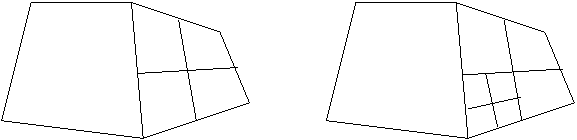
\includegraphics[width=7.6cm]{hang.pdf}
}
\end{center}
\vspace{-5mm}
\caption{Irregular meshes with one-level hanging nodes (left)
         and two-level hanging nodes (right).}
\label{fig:hang}
\end{figure}

While regular meshes are favored by theoretical
numerical analysts, meshes with hanging nodes 
yield better convergence rates. 

To illustrate this, let us consider a mesh 
consisting of four triangular 
elements (Fig. \ref{fig:hang-2} left), and 
assume that the element on the left needs to be 
refined. 

\begin{figure}[!htb]
\begin{center}
\rotatebox{0} {
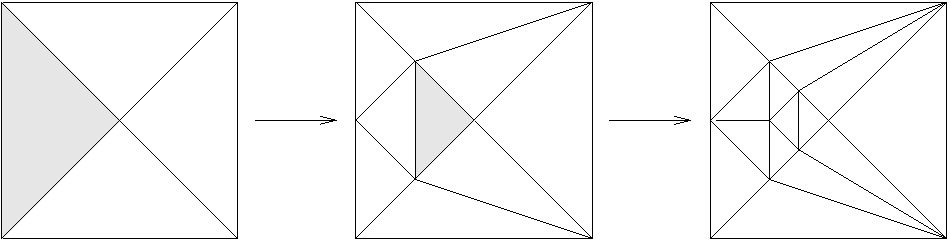
\includegraphics[width=7.6cm]{hang-2.pdf}
}
\end{center}
\vspace{-5mm}
\caption{Adaptivity with regular meshes.}
\label{fig:hang-2}
\end{figure}

If the finite element code cannot handle one-level hanging nodes,
then after splitting the element the mesh needs to be
{\em regularized}. This is done by introducing 
additional {\em forced refinements} (the four thin triangular
elements in Fig. \ref{fig:hang-2} middle). If the next 
element to be refined is the gray element in Fig.~\ref{fig:hang-2}
(middle), then the effect of mesh regularization becomes even 
worse. Recall that long thin elements in the mesh cause 
the condition number of the stiffness matrix to be unnecessarily 
high, and moreover the forced refinements are contributing unnecessary 
degrees of freedom which slow down the convergence rate of the method.


In order to avoid mesh regularization completely, one needs to resort to 
{\em arbitrary-level hanging nodes}. This technique was proposed in 
\cite{hangno-1} and extended to vector-valued finite elements in \cite{hangno-2}.
Higher-level hanging nodes typically do not appear in isotropic parts 
of the solution (such as point singularities) but they are needed to
resolve efficiently anisotropic features such as boundary or internal
layers. Such a solution
is shown in Fig. \ref{fig:atan-2}. The corresponding finite element mesh with 
three-level hanging nodes, obtained with adaptive $hp$-FEM, is shown in 
Fig. \ref{fig:atan-1}.

\begin{figure}[!htb]
\begin{center}
\rotatebox{0} {
\includegraphics[width=7.5cm]{atan-2.png}
}
\end{center}
\vspace{-5mm}
\caption{Solution with an internal layer.}
\label{fig:atan-2}
\end{figure}

\begin{figure}[!htb]
\begin{center}
\rotatebox{0} {
\includegraphics[width=6cm]{atan-1.png}
}
\end{center}
\vspace{-5mm}
\caption{Corresponding finite element mesh with three-level hanging nodes.}
\label{fig:atan-1}
\end{figure}

This example (benchmark "layer") is described in great detail in the tutorial to 
HERMES \cite{hermes}, and it is part of HERMES code repository \cite{hermes-repo}.

\subsection{Multimesh Assembling}\label{subsec:multimesh}


It is well known that in order to capture well individual behaviors 
of various solution components in multiphysics coupled problems, 
one needs to approximate them on individual meshes. 
Traditionally this has been done by decomposing the multiphysics 
problem into a series of single-physics equations via {\em operator 
splitting}, and employing an outer fixed-point iteration. 
Solution data in this type of methods is 
usually transferred between different meshes using various 
interpolation or projection techniques. These methods, however, 
are well know to suffer from loss of accuracy and even stability 
due to the interpolation or projection errors \cite{jiao}. As an 
alternative to these methods, a multimesh discretization technique 
that does not transfer solution data between meshes
was introduced recently in \cite{spacetime-1,spacetime-2}. It was shown 
in \cite{dubcova} that the multimesh discretization technique
compares favorably to methods based on intermesh data transfer.
 

Although the main focus of this paper is not on multiphysics problems, the 
multimesh assembling is extremely useful for the design 
of adaptive finite element methods that employ dynamically 
changing meshes, and therefore we find it useful to describe 
at least the main idea here. 

Assume that we have a two-equation PDE
system where the two solution components behave very differently. 
Ideally, the meshes for these two functions should be completely 
independent. However, for algorithmic reasons, we introduce a simplifying 
assumption that each of them is defined starting from a common coarse 
{\em master mesh}. and using a finite sequence of elementary refinement 
operations. The master mesh is very coarse and it may not  
be even used for discretization purposes. It serves as the top of 
a tree-like structure of meshes which is used by the multimesh 
assembling procedure. The situation is illustrated in Fig.\ref{fig:multimesh}
where the master mesh is shown on top, and two different meshes for the solution 
component are in the middle. Bottom of Fig.\ref{fig:multimesh} shows the 
{\em union mesh}, a geometrical union of all meshes in the system. 

The union mesh is never created physically in the computer memory, but its 
virtual elements guide the 
multimesh assembling algorithm. The algorithm visits all virtual elements 
of the union mesh, determines the polynomial orders for all solution components, 
transforms the integration points, evaluates the corresponding contributions 
of the bilinear and linear forms, and distributes the values into 
the stiffness matrix and right-hand side in a standard way.

\begin{figure}[h]
  \smallskip
  \centering
  \includegraphics[width=8cm]{multi.pdf}
  \vspace{-4mm}
  \caption{Example of a master mesh (top), locally refined 
           meshes for two different solution components (middle),
           and the corresponding union mesh (bottom).}
  \label{fig:multimesh}
\end{figure}

It is worth mentioning that automatic adaptivity in multimesh 
$hp$-FEM is done in such a way that all elements of all meshes 
in the system are sorted according to their error estimates, 
and thus the system of multiple meshes is handled as if it was
just one mesh. The benefit of this approach is that if some
solution component is resolved with sufficient accuracy, or it 
does not evolve in time significantly, all elements of the 
corresponding mesh are skipped, and thus one does not have to 
recalculate integral products for the corresponding block in 
the global stiffness matrix. 

\subsection{Adaptivity for Time-Dependent Problems}

In this Subsection we explain a feasible way to obtain 
adaptive finite element methods with dynamically changing meshes,
based on a combination of the multimesh assembling described
above and the so-called {\em Rothe's method}.

The Rothe's method is a natural counterpart of the widely used Method of Lines (MOL). 
Recall that the MOL performs discretization in space while 
keeping the time variable continuous, which leads to a system of ODEs in time. The Rothe's 
method, on the contrary, preserves the continuity of the spatial variable while discretizing time. 
In every time step, an evolutionary PDE is approximated by means of one or more time-independent ones. 
The number of the time-independent equations per time step is proportional to the order of accuracy of the 
time discretization method. For example, when employing the implicit Euler method, one 
has to solve one time-independent PDE per time step. The Rothe's method is fully equivalent to the 
MOL if no adaptivity in space or time takes place, but it provides a better setting 
for the application of spatially adaptive algorithms. The spatial discretization error
can be controlled by solving the time-independent equations adaptively, and the size of 
the time step can be adjusted using standard ODE techniques \cite{hairer}. 

For the sake of clarity, let us first use the 
implicit Euler discretization with a constant time step $\Delta t > 0$.
This is done by approximating the temporal derivative using a backward finite 
difference,
\begin{equation}\label{tempdir}
\frac{\partial h}{\partial t} \approx \frac{h^{n+1} - h^n}{\Delta t}.
\end{equation}
Generalizations to more sophisticated time stepping methods are straightforward
as long as the temporal partial derivative $\partial h / \partial t$ can be approximated
with some finite difference scheme as in (\ref{tempdir}). In particular, 
generalization to the second-order Crank-Nicolson scheme is very simple 
as it is just an arithmetic average of the implicit and explicit Euler methods.  

Using the backward finite difference (\ref{tempdir}), equation (\ref{rich-final}) becomes

$$
\left(C(h^{n+1})
+ \frac{\theta}{\theta_S} S \right) \frac{h^{n+1} - h^n}{\Delta t}
- \nabla \cdot (K(h^{n+1})\nabla h^{n+1})
$$
\begin{equation}\label{rich-final-2}
 - \frac{\partial K(h^{n+1})}{\partial z} = 0.
\end{equation}
Here $h^0$ enters through the initial condition 

\begin{equation}
  h(x, z, 0) = h^0(x,z),
\end{equation}
$h^n$ is known from the previous time step, 
and $h^{n+1}$ needs to be computed. The weak formulation of (\ref{rich-final-2})
is derived in a standard way. The discrete problems are systems of nonlinear
algebraic equations and we solve them using the standard Newton's method. 
For this, in addition to $C(h)$, $K(h)$ and $\partial K(h) / \partial h$ we also 
need to know $\partial C(h) / \partial h$ and $\partial^2 K(h) / \partial h^2$.


By $\tau_0$ let us denote a uniform coarse mesh covering the computational domain $\Omega$. This
mesh is used as the initial mesh for automatic adaptivity in every time step.
The first approximation $h^1(\bfx) \approx h(x, z, \Delta t_1)$ is computed adaptively 
in $k_1$ steps, starting from the 
mesh $\tau_0$ and using intermediate approximations $h^{1,1}$, $h^{1,2}$, $\ldots$, $h^{1,k_1} = h^1$ 
on meshes $\tau_{1,1}$, $\tau_{1,2}$, $\ldots$, $\tau_{1,k_{1}} = \tau_{1}$. The number $k_1$ depends 
on a user-defined tolerance $TOL_s$ for the spatial error. 

At the beginning of the $(n+1)$st time step, the approximation $h^n$ is defined on a locally 
refined mesh $\tau_n$ that was constructed adaptively in the $n$th step.
(The only exception is $h^0$ which is defined on the coarse mesh $\tau_0$.)
The unknown $h^{n+1}$ is computed adaptively in $k_{n+1}$ steps starting from the 
mesh $\tau_0$ and using intermediate approximations $h^{n+1,1}$, $h^{n+1,2}$, $\ldots$, $h^{n+1,k_{n+1}} = h^{n+1}$ 
on meshes $\tau_{n+1,1}$, $\tau_{n+1,2}$, $\ldots$, $\tau_{n+1,k_{n+1}} = \tau_{n+1}$. 
Note that in the m-th adaptivity step, the functions $h^n$ and $h^{n+1, m}$ are defined on 
different meshes $\tau_n$ and $\tau_{n+1,m}$ which were obtained 
from the coarse mesh $\tau_0$ through finite sequences of mutually independent 
local refinements. In order to perform assembling in this situation, we employ the 
multimesh $hp$-FEM that was described in Subsection \ref{subsec:multimesh}.

Adaptive time integration is typically carried out using a pair of 
methods that provide at the end of each time step two approximations 
with different orders of accuracy. In every time step, the difference between the pair of 
results provides an estimate of the local truncation error that is used to adapt the time 
step. These methods may be either embedded Runge-Kutta
methods, backward difference methods, or others \cite{hairer}. 




\section{Open Source Project HERMES}
\label{sec:hermes}

All computations that have been presented in this paper so far 
were performed using HERMES \cite{hermes}, 
an open source C++ library for rapid development of space- and 
space-time adaptive $hp$-FEM solvers, developed by the $hp$-FEM group 
at the University of Nevada, Reno.  

The software utilizes a number of novel mathematical methods and 
algorithms including finite elements based on generalized eigenfunctions 
of PDE operators \cite{eigen,hermite}, 
PDE-independent $hp$-adaptivity algorithms \cite{pdeindep}, 
$hp$-FEM approximations with arbitrary-level hanging nodes \cite{hangno-1,hangno-2}, 
adaptive multimesh $hp$-FEM  for monolithic discretization of 
multiphysics problems, and
space-time adaptive $hp$-FEM with dynamical meshes for time-dependent PDE problems 
\cite{spacetime-1,spacetime-2}. 

The library can be employed to solve various PDE problems ranging 
from stationary linear equations to complex 
time-dependent nonlinear multiphysics PDE systems. The code repository \cite{hermes-repo}
accessible on the project home page contains many examples from various 
engineering and scientific areas including civil, mechanical, 
electrical and nuclear engineering, computational fluid dynamics, 
quantum chemistry, and hydro\-lo\-gy.

\subsection{User Documentation}

The User Documentation %\footnote{http://hpfem.org/hermes2d/doc/index.html} 
written in Sphinx
is accessible on the project home page. It begins with an Introduction that explains the 
philosophy of the library, its mathematical background, and installation
on various hardware platforms including Linux, Windows Cygwin, Windows MSVC,
and MAC OS. 

The second section is introducing the user to Git. It explains how to 
clone the HERMES code repository \cite{hermes-repo}, customize Git via the .gitconfig file, 
create a local branches, make and commit changes, create and send patches,
and use Github for sharing code. 

The next part of the User Documentation is the Tutorial that is split 
into 10 sections:

\begin{enumerate}
\item Linear Problems.
\item Nonlinear Problems.
\item Time-Dependent Problems.
\item Adaptive Solution of Linear Problems.
\item Adaptive Solution of Nonlinear Problems.
\item Adaptive Solution of Time-Dependent Problems.
\item Eigenvalue Problems.
\item FVM and DG.
\item Using Trilinos.
\item Miscellaneous Techniques.
\end{enumerate}
The last two sections of the User Documentation contain 
a detailed description of about twenty benchmark problems
with known analytical solutions including convergence studies, 
and about twenty advanced examples. 

\subsection{An Example}

In order to utilize the library's functionality, the user has 
to write a custom C++ application. For typical problems, these 
applications are very simple. Let us demonstrate this on 
the adaptive example that was used in Section \ref{sec:hpfem}.
The following code snippets are part of the main.cpp file 
from benchmark "lshape" that can be retrieved from HERMES
code repository \cite{hermes-repo}. 

This problem comes with an exact solution (not shown here)
that is instantiated as follows,

\begin{code}
  CustomExactSolution exact_sln(&mesh);
\end{code}
The exact solution is used to define Dirichlet 
boundary conditions,

\begin{code}
  // Initialize boundary conditions
  DefaultEssentialBCNonConst 
    bc_essential(BDY_DIRICHLET, &exact_sln);
  EssentialBCs bcs(&bc_essential);
\end{code}
A predefined weak formulation is used for the Laplace equation,

\begin{code}
  // Initialize the weak formulation.
  DefaultWeakFormLaplace wf;
\end{code}
Weak forms in HERMES can be real or complex valued,
and there are two types of them -- {\em matrix forms} and
{\em vector forms}. 

Matrix forms can be used to represent 
\begin{itemize}
\item bilinear forms in linear problems, 
\item bilinear forms in generalized eigenproblems,
\item Jacobian forms in nonlinear problems.
\end{itemize}
Vector forms are used to define

\begin{itemize}
\item linear forms in linear problems,
\item residuals for nonlinear problems.
\end{itemize}
After that the problem 
is solved using a standard sequence 
of steps. First, the mesh is loaded
as follows,

\begin{code}
  // Load the mesh.
  Mesh mesh;
  H2DReader mloader;
  mloader.load("square_quad.mesh", &mesh);
\end{code}
The {\tt H2DReader} expects the mesh in a generic
HERMES format that allows variable parameters. 
Other readers/formats are available. 

As a second step, one performs initial mesh refinements. This
step is not relevant for the example in Section 
\ref{sec:hpfem}, but in general this functionality 
is very useful. The user can call the following 
functions of the {\tt Mesh} class whose names are 
self-explanatory:

\begin{code}
Mesh::refine_element(int id, int refinement = 0);
Mesh::convert_quads_to_triangles();
Mesh::convert_triangles_to_quads();
Mesh::refine_towards_vertex(int vertex_id, int depth);
Mesh::regularize(int n);
Mesh::unrefine_element(int id);
Mesh::unrefine_all_elements();
\end{code}
Next, one creates a finite element space,
\begin{code}
  // Create an H1 space with default shapeset.
  H1Space space(&mesh, &bcs, P_INIT);
\end{code}
Here, {\tt P\_INIT} is an initial polynomial degree 
of mesh elements which currently can be an integer
between one and ten. Other admissible spaces in
addition to {\tt H1Space} are {\tt HcurlSpace},
{\tt HdivSpace} and {\tt L2Space}. In vector-valued
PDE problems, each solution component can have 
a different space.

After defining spaces for all solution components, 
one selects a matrix solver. The options 
currently available include MUMPS, PETSc, UMFpack, SUPERLU, 
Trilinos, and a variety of Python solvers available through 
an interface to Scipy \cite{scipy}. 

For adaptive computations, one needs to specify a refinement 
selector that manages the selection of element refinement 
candidates during adaptivity, as it was described in 
\ref{subsec:cand}. In the example in Section 
\ref{sec:hpfem} we use an {\tt H1ProjBasedSelector}:

\begin{code}
  // Initialize refinement selector.
  H1ProjBasedSelector selector(CAND_LIST, CONV_EXP, 
                               H2DRS_DEFAULT_ORDER);
\end{code}
Here, {\tt CAND\_LIST} defines a set of element refinement candidates.
There are eight options:
\begin{itemize}
\item {\tt P\_ISO}: Only $p$-refinements allowed. Different directional 
      polynomial degrees on quadrilateral elements not allowed. 
\item {\tt P\_ANISO}: Only $p$-refinements allowed. Different directional 
      polynomial degrees on quadrilateral elements are allowed. 
\item {\tt H\_ISO}: Only $h$-refinements allowed. Anisotropic refinements
      of quadrilateral elements not allowed. 
\item {\tt H\_ANISO}: Only $h$-refinements allowed. Anisotropic refinements
      of quadrilateral elements are allowed. 
\item {\tt HP\_ISO}: $hp$-refinements are allowed. They can be isotropic 
      both in $h$ and $p$.
\item {\tt HP\_ANISO\_P}: $hp$-refinements are allowed. They can be anisotropic 
      in $p$ and isotropic in $h$.
\item {\tt HP\_ANISO\_H}: $hp$-refinements are allowed. They can be isotropic 
      in $p$ and anisotropic in $h$.
\item {\tt HP\_ANISO}: $hp$-refinements are allowed. They can be anisotropic 
      in $p$ and anisotropic in $h$. 
\end{itemize}
Note that the last option, {\tt HP\_ANISO} is the most general $hp$-adaptivity
scheme in HERMES with the most refinement candidates per element. Accordingly,
the selection process takes most time. Therefore, this option should only be 
used in problems with genuinely anisotropic solutions. 

Other parameters for automatic adaptivity are entered through the 
structure {\tt AdaptivityParamType}:

\begin{code}
  // Initialize adaptivity parameters.
  AdaptivityParamType apt(ERR_STOP, NDOF_STOP, 
                          THRESHOLD, STRATEGY, 
                          MESH_REGULARITY);
\end{code}
The user-defined constant {\tt ERR\_STOP} defines the level of 
relative error estimate in percent when the computationa will stop. 
{\tt NDOF\_STOP} is the threshold for the number of degrees of freedom 
when the adaptivity will stop. The other two parameters, {\tt THRESHOLD}
and {\tt STRATEGY} are determining the behavior of the adaptivity 
algorithm and their meaning can be found in the User Documentation.
{\tt MESH\_REGULARITY} determines the maximum level of hanging nodes
in the mesh. Regular meshes are not supported in HERMES due to their 
notoriously bad performance. By specifying {\tt MESH\_REGULARITY = -1},
one allows arbitrary-level hanging nodes (cf. \ref{subsec:hang}).

The adaptivity loop follows. Its first step is to 
refine the mesh globally in both $h$ and $p$ and 
compute a reference solution,

\begin{code}
  // Construct globally refined reference 
  // mesh and setup reference space.
  Space* ref_space 
    = Space::construct_refined_space(&space);

  // Assemble the reference problem.
  info("Solving on reference mesh.");
  bool is_linear = true;
  DiscreteProblem* dp 
    = new DiscreteProblem(&wf, ref_space, is_linear);
  dp->assemble(matrix, rhs);

  // Solve the linear system of the reference problem.
  //  If successful, obtain the solution.
  Solution ref_sln;
  if(solver->solve()) Solution::vector_to_solution(
    solver->get_solution(), ref_space, &ref_sln);
  else error ("Matrix solver failed.\n");
\end{code}
In the next step the reference solution is projected on
the coarse mesh to obtain a low-order part
for error estimation,

\begin{code}
  // Project the fine mesh solution on the coarse mesh.
  Solution sln;
  info("Projecting reference solution on coarse mesh.");
  OGProjection::project_global(&space, 
    &ref_sln, &sln, matrix_solver);
\end{code}
With the solution pair we can proceed to error 
estimation,

\begin{code}
  // Calculate element errors and total error estimate.
  info("Calculating error estimate and exact error.");
  Adapt* adaptivity = new Adapt(&space);
  double err_est_rel 
    = adaptivity->calc_err_est(&sln, &ref_sln) * 100;
\end{code}
Finally, with an a-posteriori error estimate, we can 
adapt the mesh:

\begin{code}
  // If err_est too large, adapt the mesh.
  if (err_est_rel < ERR_STOP) done = true;
  else
  {
    info("Adapting coarse mesh.");
    done = adaptivity->adapt(&selector, THRESHOLD, 
                       STRATEGY, MESH_REGULARITY);

    // Increase the counter of performed 
    // adaptivity steps.
    if (done == false)  as++;
  }
  if (Space::get_num_dofs(&space) >= NDOF_STOP) 
    done = true;
\end{code}
For more details we refer to the 
Sphinx tutorial to HERMES that is available on the 
project home page \cite{hermes}. 

\subsection{Interactive Web Accessibility}
\label{sec:onlinelab}

HERMES can be used remotely within the FEMhub Online Numerical Methods Laboratory
\cite{onlinelab} where anyone can create a free account and compute remotely 
through the web browser window. FEMhub \cite{femhub} is an open source distribution 
of finite element codes with a unified Python interface.
Besides HERMES it contains several other open source finite element and finite volume 
codes such FiPy \cite{fipy}, Phaml \cite{phaml}, and SfePy \cite{sfepy}.
It contains a large number of additional scientific computing and visualization 
tools such Numpy, Pysparse, Sympy, Mayavi. Matplotlib and others.   
The Online Numerical Methods Laboratory is based on ExtJS and powered 
by UNR high-performance computing facilities. The user can also connect 
it to his/her own computing servers.  

\section{Open Source Project AGROS}
\label{sec:agros}

AGROS (http://hpfem.org/agros2d) is a multiplatform C++ application for the solution 
of single and multiphysics PDE problems based on the HERMES library. AGROS provides 
an advanced graphical user interface (GUI), interactive geometry modeling and CAD import, 
automatic meshing, and a number of advanced visualization and postprocessing features (see Fig.~\ref{fig:agros}). 
The code is being developed by an engineering research group at the University of West 
Bohemia in Pilsen, Czech Republic. AGROS is distributed under the GNU General Public 
License. Currently, it supports the finite element analysis of electrostatic fields,
electric current fields, magnetic fields (steady state, harmonic and transient analysis),
heat transfer (steady state and transient analysis), basic fluid mechanics and linear 
elasticity (in development). A Richards module for variably saturated Darcian %odstranil jsem groundwater
flow is currently in development. 

\begin{figure*}[!ht]
\begin{center}
\includegraphics[height=8cm]{agros.png}
\end{center}
\vspace{-4mm}
\caption{Sample snapshot of AGROS on Mac OS X. An electromagnetic 
         simulation is shown, but a Richards module is in development.}
\label{fig:agros}
\end{figure*}



\section*{Acknowledgment}

The first author gratefully acknowledges the financial support
of the Grant Agency of the Academy of Sciences of the Czech 
Republic under Grant No. IAA100760702. The second author
was supported with a Grant of the Czech Ministry of Agriculture No.
QH 91247. 

%% The Appendices part is started with the command \appendix;
%% appendix sections are then done as normal sections
%% \appendix

%% \section{}
%% \label{}

%% References
%%
%% Following citation commands can be used in the body text:
%% Usage of \cite is as follows:
%%   \cite{key}         ==>>  [#]
%%   \cite[chap. 2]{key} ==>> [#, chap. 2]
%%

%% References with bibTeX database:

%\section*{References}

\bibliographystyle{elsarticle-num}
\begin{thebibliography}{00}

\bibitem{babuska1}
I. Babuska, B.Q. Guo: The $h$, $p$ and $hp$ Version of the Finite Element Method: Basic Theory and Applications, 
Advances in Engineering Software, Volume 15, Issue 3-4, 1992.

    \bibitem{alt-luckhaus} H. W. Alt, S. Luckhaus: Quasilinear Elliptic-Parabolic Differential Equations, Mathematische Zeitschrift 183 (1983) 311-341.

\bibitem{v-v}
I. Babuska et al: Verification and Validation in Computational Engineering and Science: Basic Concepts,
Computer Methods in Applied Mechanics and Engineering 193 (2004), 4057-4066.

\bibitem{celia}
M. A. Celia, E. T. Bouloutas, R. L. Zarba: A General Mass-Conservative Numerical Solution for the Unsaturated Flow Equation, Water Resources Research 26 (1990) 1483-1496.

    \bibitem{cools}
    R. Cools: Encyclopaedia of Cubature Formulas, {\tt http://nines.cs.kuleuven.be//research/ecf/}.

\bibitem{dubcova}
L. Dubcova, P. Solin, G. Hansen, H. Park: Comparison of Multimesh hp-FEM to Interpolation and 
Projection Methods for Spatial Coupling of Reactor Thermal and Neutron Diffusion Calculations, 
submitted to J. Comput. Phys.

\bibitem{kees3}
M. W. Farthing, C. E. Kees, T. S. Coffey, C. T. Kelley, C. T. Miller: Efficient Steady-State Solution Techniques for Variably Saturated Groundwater Flow, Advances in Water Resources 26 (2003) 833-849.

\bibitem{kuraz-jcam}  M. Kuraz, P. Mayer, M. Leps, D. Trpkosova: An Adaptive Time Discretization of the Classical and the Dual Porosity Model of Richards Equation, Journal of Computational and 
Applied Mathematics 233 (2010), 3167-3177

\bibitem{femhub}
FEMhub, an Open Source Distribution of Free Scientific Computing Codes 
with a Unified Python Interface, http://femhub.org/.

\bibitem{onlinelab}
FEMhub Online Numerical Methods Laboratory, http://lab.femhub.org/.

\bibitem{fipy}
FiPy, A Finite Volume PDE Solver Using Python, http://www.ctcms.nist.gov/fipy/.

\bibitem{forsyth}
P. Forsyth, M. Kropinksi: Monotonicity Considerations for Saturated–
Unsaturated Subsurface Flow, SIAM J. Sci. Comput. 18 (5) (1997) 1328-1354.

    \bibitem{gardner} W. R. Gardner: Some Steady State Solutions of the Unsaturated Moisture Flow Equation with Application to Evaporation from a Water Table, Soil Science 85 (1958) 228-232.

\bibitem{hairer}
E. Hairer, G, Wanner:
Solving Ordinary Differential Equations II: Stiff and Differential-Algebraic Problems,
2nd Edition, Springer Series in Mathematics, 1996.

\bibitem{hermes}
HERMES, a C++ Library for Rapid Development of Space- and Space-Time Adaptive $hp$-FEM Solvers,
http://hpfem.org/.

\bibitem{hermes-repo}
HERMES Code Repository: http://git.hpfem.org/hermes.git.

    \bibitem{huyakorn1} P. S. Huyakorn, S. D. Thomas, B. M. Thompson: Techniques for Making Finite Elements Competitive in Modeling Flow in Variably Saturated Porous Media, Water Resources Research 20(8) (1984) 1099-1115.

    \bibitem{huyakorn2} P. S. Huyakorn, E. P. Springer, V. Guvanasen, T. D. Wadsworth: A Three Dimensional Finite Element Model for Simulating Water Flow in Variably Saturated Porous Media, Water Resources Research 22(13) (1986) 1790-1808.

\bibitem{jiao} X. Jiao and M. T. Heath: Common-Refinement-Based Data Transfer Between Non-Matching Meshes in
Multiphysics Simulations. Internat. J. Numer. Methods Engrg., 61(14):2402–2427, 2004.

    \bibitem{kees}
    C.E. Kees, M.W. Farthing, C.N. Dawson.
    Locally Conservative, Stabilized Finite Element Methods for Variably Saturated Flow.
    Comput. Methods Appl. Mech. Engrg. 197 (2008) 4610-4625.

    \bibitem{unsat-prop} V. Kuraz:
    Soil Properties and Water Regime of Reclaimed Surface Dumps in the
    North Bohemia Brown-coal Region -- a Field Study,
    Waste Management 21 (2001) 147-151.


%\bibitem{kus}
%P. Kus: The Solution of Convection-Diffusion Equations Using Adaptive Higher-Order 
%Methods in Both Space and Time. Master's Thesis, Charles University, Prague, 2006.


\bibitem{kees2}
C.T. Miller, M.W. Farthing, C.E. Kees, C.T. Kelley:
Higher Order, Locally Conservative Temporal Integration Methods for Modeling Multiphase Flow in Porous Media, Developments in Water Science 47 (2002) 249-256.

    \bibitem{mualem}
    Y. Mualem: A New Model for Predicting the Hydraulic Conductivity of Unsaturated Porous Media, Water Resources Research 12 (1976) 513-522.

    \bibitem{neuman1} S. P. Neuman, P. A. Witherspoon: Finite Element Method Analyzing Steady Seepage with a Free Surface, Water Resources Research 6(3) (1970) 889-897.

    \bibitem{neuman2} S. P. Neuman, P. A. Witherspoon: Analysis of Nonsteady Flow with a Free Surface Using the Finite Element Method, Water Resources Research 7(3) (1971) 611-623.

    \bibitem{neuman3} S. P. Neuman: Saturated-Unsaturated Seepage by Finite Elements, Journal of the Hydraulics Division 12 (1973) 2233-2250.


    \bibitem{pech} P. Pech: Determination of Skin Factor by Means of the Intersection Time from the Early-portion of Pumping Test, Journal of Environmental Hydrology 11 (2003) 1-9.

\bibitem{phaml}
Phaml, a Fortran 90 code using adaptive refinement, multigrid and parallel computing to solve 2-D linear elliptic PDEs, http://math.nist.gov/phaml/.


    \bibitem{richards} L.A. Richards, Physics 1 - DOI:10.1063/1.1745010 (1931) 318-333.
Gaddafi also appointed Ali Abdussalam Treki, a senior Libyan diplomat, to be his country's new envoy to the UN after the entire Libyan delegation in New York deserted Gaddafi in support of Libya's protesters.


    \bibitem{scipy} Scipy: Open Source Library of Scientific Tools, {\tt http://www.scipy.org/}.

\bibitem{sfepy}
SfePy: Simple Finite Elements in Python, http://code.google.com/p/sfepy/.

    \bibitem{pdeindep}
    P. Solin, D. Andrs, J. Cerveny, M. Simko: PDE-Independent Adaptive hp-FEM
    Based on Hierarchic Extension of Finite Element Spaces, J. Comput. Appl.
    Math. 233 (2010) 3086-3094

    \bibitem{hangno-1}
    P. Solin, J. Cerveny, I. Dolezel: Arbitrary-Level Hanging Nodes and Automatic
    Adaptivity in the hp-FEM, Math. Comput. Simul. 77 (2008), 117 - 132.

    \bibitem{sode} P. Solin, L. Demkowicz: Goal-Oriented hp-Adaptivity for 
    Elliptic Problems, Comput. Methods Appl. Mech. Engrg. 193 (2004), 449 - 468.

    \bibitem{hangno-2}
    P. Solin, L. Dubcova, J. Cerveny, I. Dolezel: Adaptive hp-FEM with Arbitrary-Level
    Hanging Nodes for Maxwell's Equations, Advances in Applied Mathematics and Mechanics,
    Vol. 2, No. 4, 2010, pp. 518 - 532.

%    \bibitem{thermoel}
%    P. Solin, J. Cerveny, L. Dubcova, D. Andrs. Monolithic Discretization of Linear
%    Thermoelasticity Problems via Adaptive Multimesh hp-FEM, J. Comput. Appl. Math 234
%    (2010) 2350 - 2357.

    \bibitem{spacetime-1}
    P. Solin, L. Dubcova, J. Kruis: Adaptive hp-FEM with Dynamical Meshes for Transient Heat and Moisture Transfer Problems, J. Comput. Appl. Math. 233 (2010) 3103-3112.

    \bibitem{spacetime-2}
    P. Solin, L. Dubcova, J. Kruis: Adaptive hp-FEM with Dynamical Meshes for Transient Heat and Moisture Transfer Problems, J. Comput. Appl. Math. 233 (2010) 3103-3112.

    \bibitem{hermite}
    P. Solin, K. Segeth: Hierarchic Higher-Order Hermite Elements on Hybrid
    Triangular/Quadrilateral Meshes, Math. Comput. Simul. (76) 2007, pp. 198 - 204.

    \bibitem{sosedo}
    P. Solin, K. Segeth, I Dolezel. {\em Higher-Order Finite Element Methods}, CHapman \& Hall / CRC Press,
    2003.

    \bibitem{eigen}
    P. Solin, T. Vejchodsky: Higher-Order Finite Elements Based on Generalized Eigenfunctions
    of the Laplacian, Int. J. Numer. Methods Engrg 73 (2007), 1374 - 1394.

%\bibitem{sphinx}
%Sphinx, a Free Open-Source SQL Full-Text Search Engine, http://www.sphinxsearch.com/.

    \bibitem{tracy1} F. T. Tracy: Clean Two- and Three-Dimensional Analytical Solutions of Richards Equation for Testing 
    Numerical Solvers, Water Resources Research 42(8) ( 2006).

% tahle druha citace tracyho bude asi zbytecna
\bibitem{tracy2} F. T. Tracy: Three-Dimensional Analytical Solutions of Richards’ Equation for a Box-Shaped Soil 
    Sample with Piecewise-Constant Head Boundary Conditions on the Top, Journal of Hydrology 336(3-4) (2007) 391-400.


    \bibitem{vangenuchten}
    M. T. H. van Genuchten: A Closed-form Equation for Predicting the Hydraulic Conductivity of Unsaturated Soils, Journal of Soil Science, 44(5) (1980) 892-898.

\bibitem{rawra} RAWRA -- Radioactive Waste Repository Authority of the Czech Republic, http://www.rawra.cz

\bibitem{ross} P. J. Ross: Cubic approximation of hydraulic properties for simulations of unsaturated flow, Water Resour. Res., 28(10) (1992), 2617-2620.

\bibitem{simunek} J. Simunek, K. Huang, M. Sejna, and M. T. van Genuchten: The HYDRUS-1D Software Package for Simulating the One-Dimensional
Movement of Water Heat, and Multiple Solutes Variably Saturated Media, Version 1.0, U.S. Salinity Lab., U.S. Dep. of Agric.,
Riverside, Calif., (1997)

\bibitem{miller} C. T. Miller, G. A. Williams, C. T. Kelley, M. D. Tocci: Robust Solution of Richards Equation for Nonuniform Porous Media, Water Resour. Res. 34(10) (1998), 2599-2610.

\bibitem{vogel} T. Vogel, M. Th. van Genuchten, M. Cislerova: Effect of the Shape of the Soil Hydraulic Functions Near Saturation on
Variably-Saturated Flow Predictions, Advances in Water Resources 24 (2001) 133-144.

\bibitem{kees-time-integ} C.E. Kees, C.T. Miller: Higher order time integration methods for two-phase flow, Advances in Water Resources 25(2002) 159-177.

%\bibitem{sdirk} F. Ismail, R.A. Al-Khasawneh, M. Suleiman: Embedded Singly Diagonally Implicit Runge-Kutta-Nystr\'om General Method (3,4) in (4,5) for Solving Second Order IVPs, International Journal of Applied Mathematics 37(2007)


 \end{thebibliography}


\end{document}

%%
%% End of file `elsarticle-template-num.tex'.
